\section{Border effects}
\subsection{Estimation design}
\begin{table}[H]
	\centering		
    \caption{Cross-border shopping - Overall}
    \label{tab: app_border_eff_spectest_cbshopping_overall}
	\begin{spacing}{1.1}
        \scalebox{0.97}{
        \begin{tabular}{lrrrr} \toprule
            &   \multicolumn{2}{c}{Total} & \multicolumn{2}{c}{Share} 
                \\ \cmidrule(lr){2-3} \cmidrule(lr){4-5} 
            Store region & Transaction & Sales & Transaction & Sales \\ \midrule
		    Belgium&55,221,132&174,211,718&0.979&0.978\\
France&216,535&797,661&0.004&0.004\\
The Netherlands&522,119&1,408,998&0.009&0.008\\
Other foreign&462,753&1,490,103&0.008&0.008\\
Unknown&11,331&138,077&0.000&0.001\\
\bottomrule

	    \end{tabular}}
    \end{spacing}
    \parbox{\textwidth}{
        \begin{spacing}{1} 
            {\footnotesize 
            \textit{Notes}: This table provides the total number of transactions, the total expenditure, the share in the total number of transactions and the share in total expenditure for stores located in Belgium, France, the Netherlands, in another country and for stores which we cannot locate. To obtain these numbers we include all purchases made by Belgian households for the full sample period. Expenditure is expressed in EUR.}
        \end{spacing}}
\end{table}

\begin{figure}[H]
    \centering
    \caption{Cross-border shopping - Distance to the border}
    \label{fig: app_border_eff_spectest_cbshopping_distance}
    \begin{subfigure}[t]{.49\textwidth}
         \centering
         \caption{France - Propensity}
         \scalebox{0.45}{% Created by tikzDevice version 0.12.3.1 on 2022-08-25 11:14:06
% !TEX encoding = UTF-8 Unicode
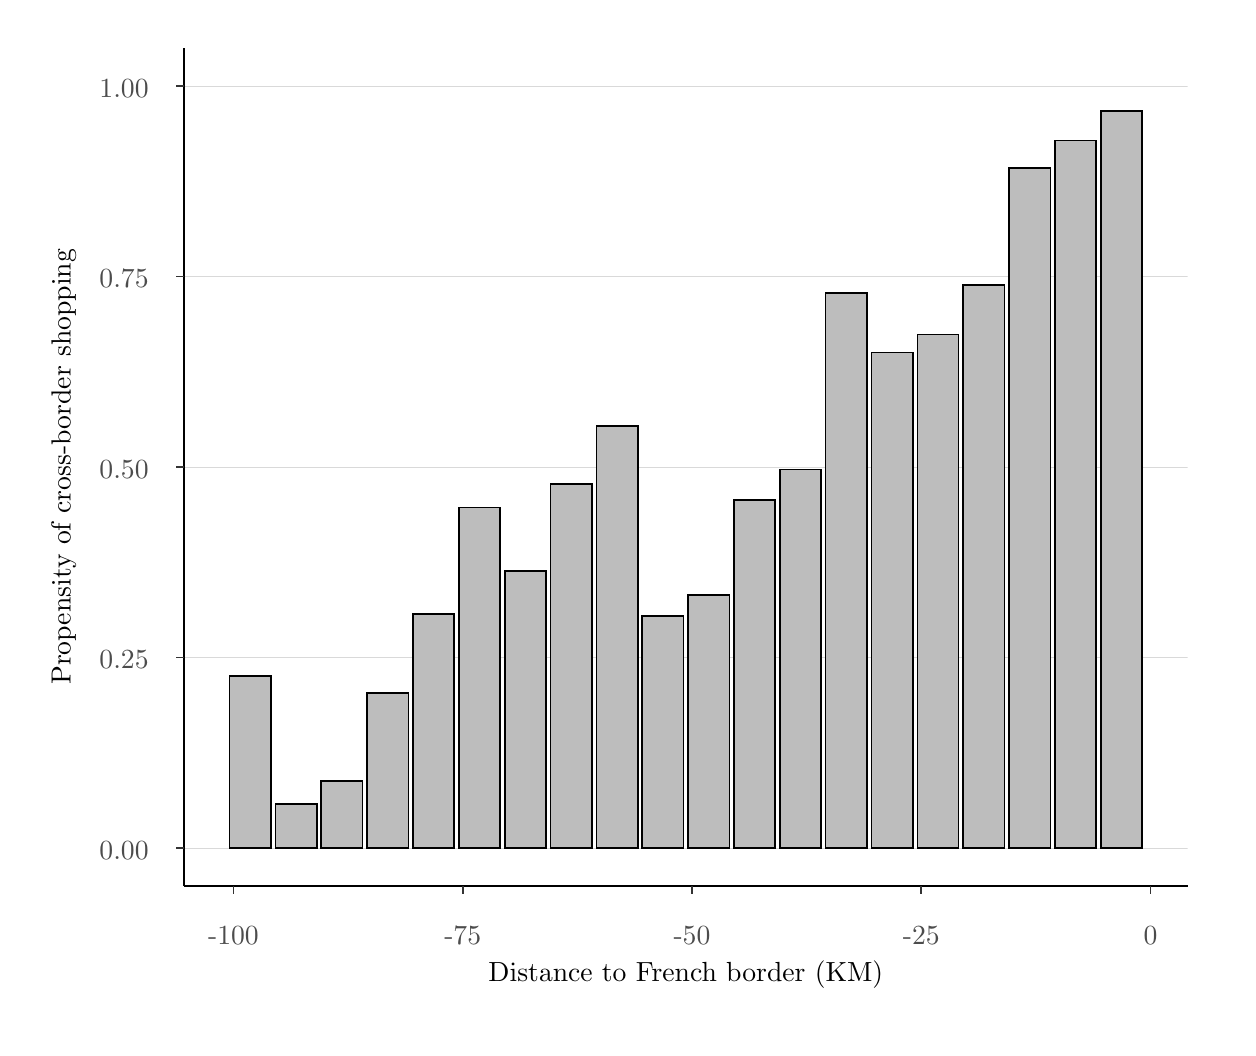
\begin{tikzpicture}[x=1pt,y=1pt]
\definecolor{fillColor}{RGB}{255,255,255}
\path[use as bounding box,fill=fillColor,fill opacity=0.00] (0,0) rectangle (433.62,361.35);
\begin{scope}
\path[clip] (  0.00,  0.00) rectangle (433.62,361.35);
\definecolor{drawColor}{RGB}{255,255,255}
\definecolor{fillColor}{RGB}{255,255,255}

\path[draw=drawColor,line width= 0.6pt,line join=round,line cap=round,fill=fillColor] ( -0.00,  0.00) rectangle (433.62,361.35);
\end{scope}
\begin{scope}
\path[clip] ( 56.47, 51.15) rectangle (419.17,354.12);
\definecolor{drawColor}{RGB}{255,255,255}

\path[draw=drawColor,line width= 0.3pt,line join=round] ( 56.47, 99.35) --
	(419.17, 99.35);

\path[draw=drawColor,line width= 0.3pt,line join=round] ( 56.47,168.21) --
	(419.17,168.21);

\path[draw=drawColor,line width= 0.3pt,line join=round] ( 56.47,237.07) --
	(419.17,237.07);

\path[draw=drawColor,line width= 0.3pt,line join=round] ( 56.47,305.92) --
	(419.17,305.92);

\path[draw=drawColor,line width= 0.3pt,line join=round] (115.77, 51.15) --
	(115.77,354.12);

\path[draw=drawColor,line width= 0.3pt,line join=round] (198.62, 51.15) --
	(198.62,354.12);

\path[draw=drawColor,line width= 0.3pt,line join=round] (281.46, 51.15) --
	(281.46,354.12);

\path[draw=drawColor,line width= 0.3pt,line join=round] (364.31, 51.15) --
	(364.31,354.12);
\definecolor{drawColor}{gray}{0.85}

\path[draw=drawColor,line width= 0.1pt,line join=round] ( 56.47, 64.92) --
	(419.17, 64.92);

\path[draw=drawColor,line width= 0.1pt,line join=round] ( 56.47,133.78) --
	(419.17,133.78);

\path[draw=drawColor,line width= 0.1pt,line join=round] ( 56.47,202.64) --
	(419.17,202.64);

\path[draw=drawColor,line width= 0.1pt,line join=round] ( 56.47,271.49) --
	(419.17,271.49);

\path[draw=drawColor,line width= 0.1pt,line join=round] ( 56.47,340.35) --
	(419.17,340.35);
\definecolor{drawColor}{RGB}{0,0,0}
\definecolor{fillColor}{gray}{0.74}

\path[draw=drawColor,line width= 0.6pt,line cap=rect,fill=fillColor] ( 72.95, 64.92) rectangle ( 87.86,127.13);

\path[draw=drawColor,line width= 0.6pt,line cap=rect,fill=fillColor] ( 89.52, 64.92) rectangle (104.43, 80.72);

\path[draw=drawColor,line width= 0.6pt,line cap=rect,fill=fillColor] (106.09, 64.92) rectangle (121.00, 89.10);

\path[draw=drawColor,line width= 0.6pt,line cap=rect,fill=fillColor] (122.66, 64.92) rectangle (137.57,120.87);

\path[draw=drawColor,line width= 0.6pt,line cap=rect,fill=fillColor] (139.23, 64.92) rectangle (154.14,149.51);

\path[draw=drawColor,line width= 0.6pt,line cap=rect,fill=fillColor] (155.80, 64.92) rectangle (170.71,187.94);

\path[draw=drawColor,line width= 0.6pt,line cap=rect,fill=fillColor] (172.37, 64.92) rectangle (187.28,165.10);

\path[draw=drawColor,line width= 0.6pt,line cap=rect,fill=fillColor] (188.94, 64.92) rectangle (203.85,196.42);

\path[draw=drawColor,line width= 0.6pt,line cap=rect,fill=fillColor] (205.51, 64.92) rectangle (220.42,217.31);

\path[draw=drawColor,line width= 0.6pt,line cap=rect,fill=fillColor] (222.08, 64.92) rectangle (236.99,148.70);

\path[draw=drawColor,line width= 0.6pt,line cap=rect,fill=fillColor] (238.64, 64.92) rectangle (253.56,156.39);

\path[draw=drawColor,line width= 0.6pt,line cap=rect,fill=fillColor] (255.21, 64.92) rectangle (270.13,190.65);

\path[draw=drawColor,line width= 0.6pt,line cap=rect,fill=fillColor] (271.78, 64.92) rectangle (286.70,201.64);

\path[draw=drawColor,line width= 0.6pt,line cap=rect,fill=fillColor] (288.35, 64.92) rectangle (303.26,265.38);

\path[draw=drawColor,line width= 0.6pt,line cap=rect,fill=fillColor] (304.92, 64.92) rectangle (319.83,244.00);

\path[draw=drawColor,line width= 0.6pt,line cap=rect,fill=fillColor] (321.49, 64.92) rectangle (336.40,250.50);

\path[draw=drawColor,line width= 0.6pt,line cap=rect,fill=fillColor] (338.06, 64.92) rectangle (352.97,268.40);

\path[draw=drawColor,line width= 0.6pt,line cap=rect,fill=fillColor] (354.63, 64.92) rectangle (369.54,310.67);

\path[draw=drawColor,line width= 0.6pt,line cap=rect,fill=fillColor] (371.20, 64.92) rectangle (386.11,320.61);

\path[draw=drawColor,line width= 0.6pt,line cap=rect,fill=fillColor] (387.77, 64.92) rectangle (402.68,331.30);
\end{scope}
\begin{scope}
\path[clip] (  0.00,  0.00) rectangle (433.62,361.35);
\definecolor{drawColor}{RGB}{0,0,0}

\path[draw=drawColor,line width= 0.6pt,line join=round] ( 56.47, 51.15) --
	( 56.47,354.12);
\end{scope}
\begin{scope}
\path[clip] (  0.00,  0.00) rectangle (433.62,361.35);
\definecolor{drawColor}{gray}{0.30}

\node[text=drawColor,anchor=base east,inner sep=0pt, outer sep=0pt, scale=  1.00] at ( 43.72, 60.79) {0.00};

\node[text=drawColor,anchor=base east,inner sep=0pt, outer sep=0pt, scale=  1.00] at ( 43.72,129.65) {0.25};

\node[text=drawColor,anchor=base east,inner sep=0pt, outer sep=0pt, scale=  1.00] at ( 43.72,198.51) {0.50};

\node[text=drawColor,anchor=base east,inner sep=0pt, outer sep=0pt, scale=  1.00] at ( 43.72,267.36) {0.75};

\node[text=drawColor,anchor=base east,inner sep=0pt, outer sep=0pt, scale=  1.00] at ( 43.72,336.22) {1.00};
\end{scope}
\begin{scope}
\path[clip] (  0.00,  0.00) rectangle (433.62,361.35);
\definecolor{drawColor}{gray}{0.20}

\path[draw=drawColor,line width= 0.6pt,line join=round] ( 53.72, 64.92) --
	( 56.47, 64.92);

\path[draw=drawColor,line width= 0.6pt,line join=round] ( 53.72,133.78) --
	( 56.47,133.78);

\path[draw=drawColor,line width= 0.6pt,line join=round] ( 53.72,202.64) --
	( 56.47,202.64);

\path[draw=drawColor,line width= 0.6pt,line join=round] ( 53.72,271.49) --
	( 56.47,271.49);

\path[draw=drawColor,line width= 0.6pt,line join=round] ( 53.72,340.35) --
	( 56.47,340.35);
\end{scope}
\begin{scope}
\path[clip] (  0.00,  0.00) rectangle (433.62,361.35);
\definecolor{drawColor}{RGB}{0,0,0}

\path[draw=drawColor,line width= 0.6pt,line join=round] ( 56.47, 51.15) --
	(419.17, 51.15);
\end{scope}
\begin{scope}
\path[clip] (  0.00,  0.00) rectangle (433.62,361.35);
\definecolor{drawColor}{gray}{0.20}

\path[draw=drawColor,line width= 0.6pt,line join=round] ( 74.35, 48.40) --
	( 74.35, 51.15);

\path[draw=drawColor,line width= 0.6pt,line join=round] (157.20, 48.40) --
	(157.20, 51.15);

\path[draw=drawColor,line width= 0.6pt,line join=round] (240.04, 48.40) --
	(240.04, 51.15);

\path[draw=drawColor,line width= 0.6pt,line join=round] (322.89, 48.40) --
	(322.89, 51.15);

\path[draw=drawColor,line width= 0.6pt,line join=round] (405.73, 48.40) --
	(405.73, 51.15);
\end{scope}
\begin{scope}
\path[clip] (  0.00,  0.00) rectangle (433.62,361.35);
\definecolor{drawColor}{gray}{0.30}

\node[text=drawColor,anchor=base,inner sep=0pt, outer sep=0pt, scale=  1.00] at ( 74.35, 30.14) {-100};

\node[text=drawColor,anchor=base,inner sep=0pt, outer sep=0pt, scale=  1.00] at (157.20, 30.14) {-75};

\node[text=drawColor,anchor=base,inner sep=0pt, outer sep=0pt, scale=  1.00] at (240.04, 30.14) {-50};

\node[text=drawColor,anchor=base,inner sep=0pt, outer sep=0pt, scale=  1.00] at (322.89, 30.14) {-25};

\node[text=drawColor,anchor=base,inner sep=0pt, outer sep=0pt, scale=  1.00] at (405.73, 30.14) {0};
\end{scope}
\begin{scope}
\path[clip] (  0.00,  0.00) rectangle (433.62,361.35);
\definecolor{drawColor}{RGB}{0,0,0}

\node[text=drawColor,anchor=base,inner sep=0pt, outer sep=0pt, scale=  1.00] at (237.82, 16.79) {Distance to French border (KM)};
\end{scope}
\begin{scope}
\path[clip] (  0.00,  0.00) rectangle (433.62,361.35);
\definecolor{drawColor}{RGB}{0,0,0}

\node[text=drawColor,rotate= 90.00,anchor=base,inner sep=0pt, outer sep=0pt, scale=  1.00] at ( 15.49,202.64) {Propensity of cross-border shopping};
\end{scope}
\end{tikzpicture}
}
     \end{subfigure}
     \begin{subfigure}[t]{.49\textwidth}
         \centering
         \caption{France - Expenditure}
         \scalebox{0.45}{% Created by tikzDevice version 0.12.3.1 on 2022-08-25 11:16:46
% !TEX encoding = UTF-8 Unicode
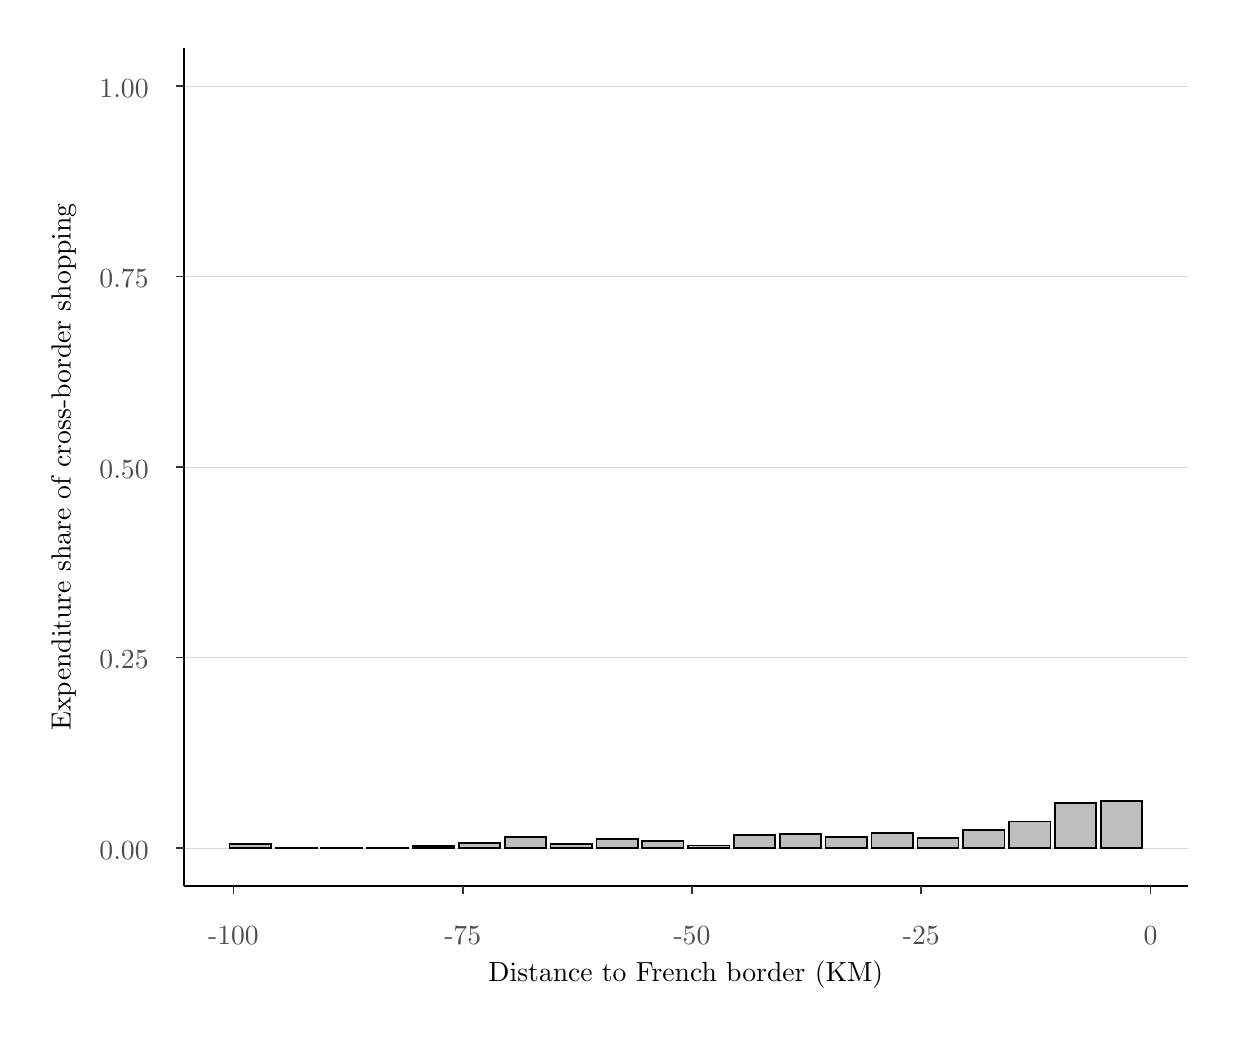
\begin{tikzpicture}[x=1pt,y=1pt]
\definecolor{fillColor}{RGB}{255,255,255}
\path[use as bounding box,fill=fillColor,fill opacity=0.00] (0,0) rectangle (433.62,361.35);
\begin{scope}
\path[clip] (  0.00,  0.00) rectangle (433.62,361.35);
\definecolor{drawColor}{RGB}{255,255,255}
\definecolor{fillColor}{RGB}{255,255,255}

\path[draw=drawColor,line width= 0.6pt,line join=round,line cap=round,fill=fillColor] ( -0.00,  0.00) rectangle (433.62,361.35);
\end{scope}
\begin{scope}
\path[clip] ( 56.47, 51.15) rectangle (419.17,354.12);
\definecolor{drawColor}{RGB}{255,255,255}

\path[draw=drawColor,line width= 0.3pt,line join=round] ( 56.47, 99.35) --
	(419.17, 99.35);

\path[draw=drawColor,line width= 0.3pt,line join=round] ( 56.47,168.21) --
	(419.17,168.21);

\path[draw=drawColor,line width= 0.3pt,line join=round] ( 56.47,237.07) --
	(419.17,237.07);

\path[draw=drawColor,line width= 0.3pt,line join=round] ( 56.47,305.92) --
	(419.17,305.92);

\path[draw=drawColor,line width= 0.3pt,line join=round] (115.77, 51.15) --
	(115.77,354.12);

\path[draw=drawColor,line width= 0.3pt,line join=round] (198.62, 51.15) --
	(198.62,354.12);

\path[draw=drawColor,line width= 0.3pt,line join=round] (281.46, 51.15) --
	(281.46,354.12);

\path[draw=drawColor,line width= 0.3pt,line join=round] (364.31, 51.15) --
	(364.31,354.12);
\definecolor{drawColor}{gray}{0.85}

\path[draw=drawColor,line width= 0.1pt,line join=round] ( 56.47, 64.92) --
	(419.17, 64.92);

\path[draw=drawColor,line width= 0.1pt,line join=round] ( 56.47,133.78) --
	(419.17,133.78);

\path[draw=drawColor,line width= 0.1pt,line join=round] ( 56.47,202.64) --
	(419.17,202.64);

\path[draw=drawColor,line width= 0.1pt,line join=round] ( 56.47,271.49) --
	(419.17,271.49);

\path[draw=drawColor,line width= 0.1pt,line join=round] ( 56.47,340.35) --
	(419.17,340.35);
\definecolor{drawColor}{RGB}{0,0,0}
\definecolor{fillColor}{gray}{0.74}

\path[draw=drawColor,line width= 0.6pt,line cap=rect,fill=fillColor] ( 72.95, 64.92) rectangle ( 87.86, 66.43);

\path[draw=drawColor,line width= 0.6pt,line cap=rect,fill=fillColor] ( 89.52, 64.92) rectangle (104.43, 64.97);

\path[draw=drawColor,line width= 0.6pt,line cap=rect,fill=fillColor] (106.09, 64.92) rectangle (121.00, 64.95);

\path[draw=drawColor,line width= 0.6pt,line cap=rect,fill=fillColor] (122.66, 64.92) rectangle (137.57, 65.12);

\path[draw=drawColor,line width= 0.6pt,line cap=rect,fill=fillColor] (139.23, 64.92) rectangle (154.14, 65.60);

\path[draw=drawColor,line width= 0.6pt,line cap=rect,fill=fillColor] (155.80, 64.92) rectangle (170.71, 66.77);

\path[draw=drawColor,line width= 0.6pt,line cap=rect,fill=fillColor] (172.37, 64.92) rectangle (187.28, 68.92);

\path[draw=drawColor,line width= 0.6pt,line cap=rect,fill=fillColor] (188.94, 64.92) rectangle (203.85, 66.44);

\path[draw=drawColor,line width= 0.6pt,line cap=rect,fill=fillColor] (205.51, 64.92) rectangle (220.42, 68.18);

\path[draw=drawColor,line width= 0.6pt,line cap=rect,fill=fillColor] (222.08, 64.92) rectangle (236.99, 67.35);

\path[draw=drawColor,line width= 0.6pt,line cap=rect,fill=fillColor] (238.64, 64.92) rectangle (253.56, 65.88);

\path[draw=drawColor,line width= 0.6pt,line cap=rect,fill=fillColor] (255.21, 64.92) rectangle (270.13, 69.59);

\path[draw=drawColor,line width= 0.6pt,line cap=rect,fill=fillColor] (271.78, 64.92) rectangle (286.70, 69.87);

\path[draw=drawColor,line width= 0.6pt,line cap=rect,fill=fillColor] (288.35, 64.92) rectangle (303.26, 68.93);

\path[draw=drawColor,line width= 0.6pt,line cap=rect,fill=fillColor] (304.92, 64.92) rectangle (319.83, 70.37);

\path[draw=drawColor,line width= 0.6pt,line cap=rect,fill=fillColor] (321.49, 64.92) rectangle (336.40, 68.51);

\path[draw=drawColor,line width= 0.6pt,line cap=rect,fill=fillColor] (338.06, 64.92) rectangle (352.97, 71.33);

\path[draw=drawColor,line width= 0.6pt,line cap=rect,fill=fillColor] (354.63, 64.92) rectangle (369.54, 74.49);

\path[draw=drawColor,line width= 0.6pt,line cap=rect,fill=fillColor] (371.20, 64.92) rectangle (386.11, 81.26);

\path[draw=drawColor,line width= 0.6pt,line cap=rect,fill=fillColor] (387.77, 64.92) rectangle (402.68, 81.95);
\end{scope}
\begin{scope}
\path[clip] (  0.00,  0.00) rectangle (433.62,361.35);
\definecolor{drawColor}{RGB}{0,0,0}

\path[draw=drawColor,line width= 0.6pt,line join=round] ( 56.47, 51.15) --
	( 56.47,354.12);
\end{scope}
\begin{scope}
\path[clip] (  0.00,  0.00) rectangle (433.62,361.35);
\definecolor{drawColor}{gray}{0.30}

\node[text=drawColor,anchor=base east,inner sep=0pt, outer sep=0pt, scale=  1.00] at ( 43.72, 60.79) {0.00};

\node[text=drawColor,anchor=base east,inner sep=0pt, outer sep=0pt, scale=  1.00] at ( 43.72,129.65) {0.25};

\node[text=drawColor,anchor=base east,inner sep=0pt, outer sep=0pt, scale=  1.00] at ( 43.72,198.51) {0.50};

\node[text=drawColor,anchor=base east,inner sep=0pt, outer sep=0pt, scale=  1.00] at ( 43.72,267.36) {0.75};

\node[text=drawColor,anchor=base east,inner sep=0pt, outer sep=0pt, scale=  1.00] at ( 43.72,336.22) {1.00};
\end{scope}
\begin{scope}
\path[clip] (  0.00,  0.00) rectangle (433.62,361.35);
\definecolor{drawColor}{gray}{0.20}

\path[draw=drawColor,line width= 0.6pt,line join=round] ( 53.72, 64.92) --
	( 56.47, 64.92);

\path[draw=drawColor,line width= 0.6pt,line join=round] ( 53.72,133.78) --
	( 56.47,133.78);

\path[draw=drawColor,line width= 0.6pt,line join=round] ( 53.72,202.64) --
	( 56.47,202.64);

\path[draw=drawColor,line width= 0.6pt,line join=round] ( 53.72,271.49) --
	( 56.47,271.49);

\path[draw=drawColor,line width= 0.6pt,line join=round] ( 53.72,340.35) --
	( 56.47,340.35);
\end{scope}
\begin{scope}
\path[clip] (  0.00,  0.00) rectangle (433.62,361.35);
\definecolor{drawColor}{RGB}{0,0,0}

\path[draw=drawColor,line width= 0.6pt,line join=round] ( 56.47, 51.15) --
	(419.17, 51.15);
\end{scope}
\begin{scope}
\path[clip] (  0.00,  0.00) rectangle (433.62,361.35);
\definecolor{drawColor}{gray}{0.20}

\path[draw=drawColor,line width= 0.6pt,line join=round] ( 74.35, 48.40) --
	( 74.35, 51.15);

\path[draw=drawColor,line width= 0.6pt,line join=round] (157.20, 48.40) --
	(157.20, 51.15);

\path[draw=drawColor,line width= 0.6pt,line join=round] (240.04, 48.40) --
	(240.04, 51.15);

\path[draw=drawColor,line width= 0.6pt,line join=round] (322.89, 48.40) --
	(322.89, 51.15);

\path[draw=drawColor,line width= 0.6pt,line join=round] (405.73, 48.40) --
	(405.73, 51.15);
\end{scope}
\begin{scope}
\path[clip] (  0.00,  0.00) rectangle (433.62,361.35);
\definecolor{drawColor}{gray}{0.30}

\node[text=drawColor,anchor=base,inner sep=0pt, outer sep=0pt, scale=  1.00] at ( 74.35, 30.14) {-100};

\node[text=drawColor,anchor=base,inner sep=0pt, outer sep=0pt, scale=  1.00] at (157.20, 30.14) {-75};

\node[text=drawColor,anchor=base,inner sep=0pt, outer sep=0pt, scale=  1.00] at (240.04, 30.14) {-50};

\node[text=drawColor,anchor=base,inner sep=0pt, outer sep=0pt, scale=  1.00] at (322.89, 30.14) {-25};

\node[text=drawColor,anchor=base,inner sep=0pt, outer sep=0pt, scale=  1.00] at (405.73, 30.14) {0};
\end{scope}
\begin{scope}
\path[clip] (  0.00,  0.00) rectangle (433.62,361.35);
\definecolor{drawColor}{RGB}{0,0,0}

\node[text=drawColor,anchor=base,inner sep=0pt, outer sep=0pt, scale=  1.00] at (237.82, 16.79) {Distance to French border (KM)};
\end{scope}
\begin{scope}
\path[clip] (  0.00,  0.00) rectangle (433.62,361.35);
\definecolor{drawColor}{RGB}{0,0,0}

\node[text=drawColor,rotate= 90.00,anchor=base,inner sep=0pt, outer sep=0pt, scale=  1.00] at ( 15.49,202.64) {Expenditure share of cross-border shopping};
\end{scope}
\end{tikzpicture}
}
     \end{subfigure}\\
     \begin{subfigure}[t]{.49\textwidth}
         \centering
         \caption{The Netherlands - Propensity}
         \scalebox{0.45}{\input{figures/descriptives/P1_2_1_1_2_crossborder_nl_prop.tex}}
     \end{subfigure}
     \begin{subfigure}[t]{.49\textwidth}
         \centering
         \caption{The Netherlands - Expenditure}
         \scalebox{0.45}{% Created by tikzDevice version 0.12.3.1 on 2022-08-25 11:17:47
% !TEX encoding = UTF-8 Unicode
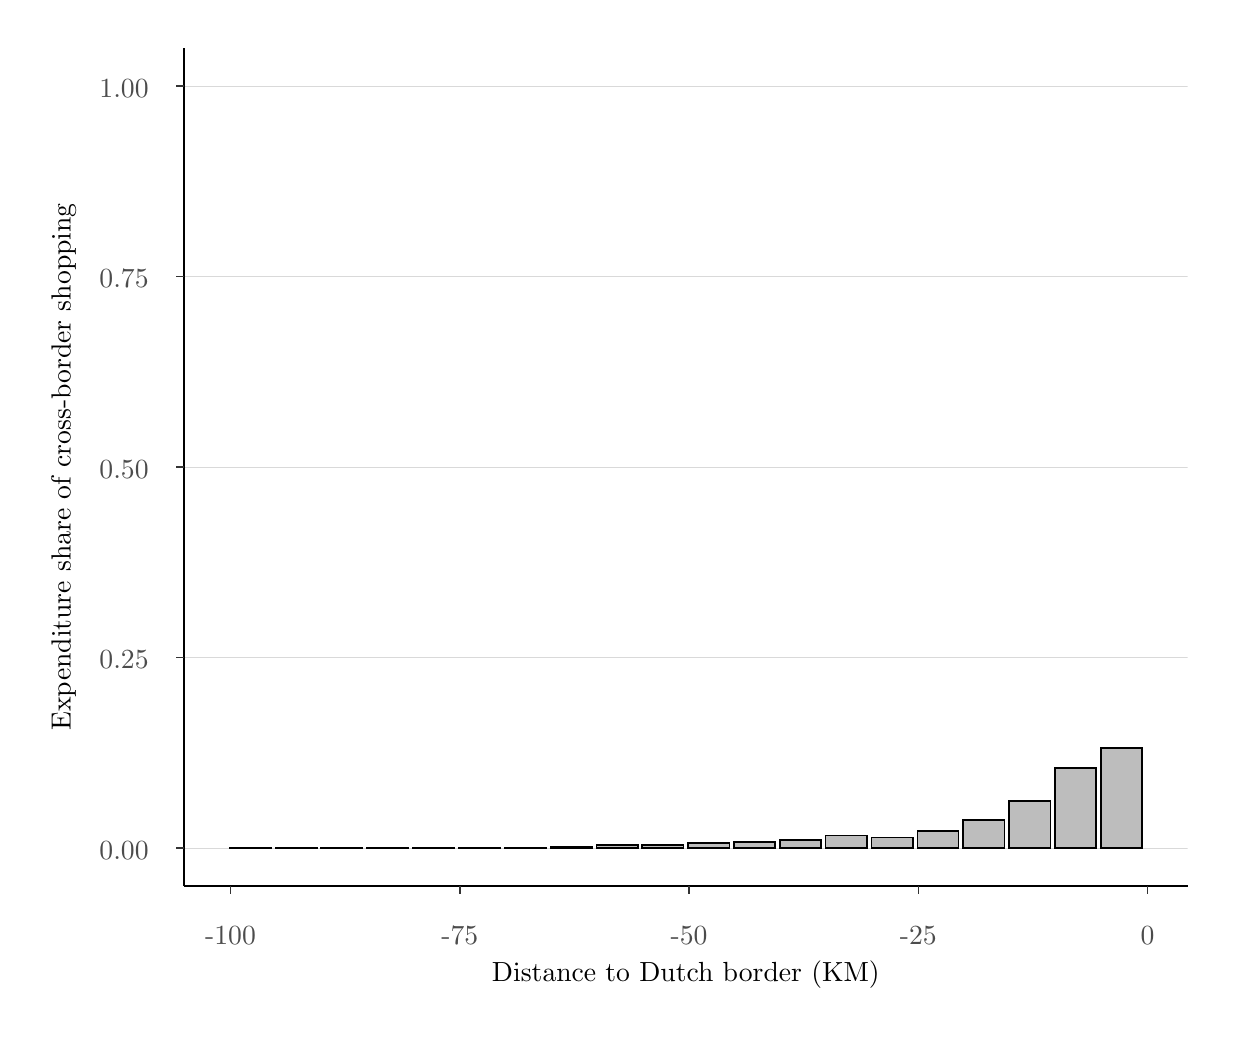
\begin{tikzpicture}[x=1pt,y=1pt]
\definecolor{fillColor}{RGB}{255,255,255}
\path[use as bounding box,fill=fillColor,fill opacity=0.00] (0,0) rectangle (433.62,361.35);
\begin{scope}
\path[clip] (  0.00,  0.00) rectangle (433.62,361.35);
\definecolor{drawColor}{RGB}{255,255,255}
\definecolor{fillColor}{RGB}{255,255,255}

\path[draw=drawColor,line width= 0.6pt,line join=round,line cap=round,fill=fillColor] ( -0.00,  0.00) rectangle (433.62,361.35);
\end{scope}
\begin{scope}
\path[clip] ( 56.47, 51.15) rectangle (419.17,354.12);
\definecolor{drawColor}{RGB}{255,255,255}

\path[draw=drawColor,line width= 0.3pt,line join=round] ( 56.47, 99.35) --
	(419.17, 99.35);

\path[draw=drawColor,line width= 0.3pt,line join=round] ( 56.47,168.21) --
	(419.17,168.21);

\path[draw=drawColor,line width= 0.3pt,line join=round] ( 56.47,237.07) --
	(419.17,237.07);

\path[draw=drawColor,line width= 0.3pt,line join=round] ( 56.47,305.92) --
	(419.17,305.92);

\path[draw=drawColor,line width= 0.3pt,line join=round] (114.72, 51.15) --
	(114.72,354.12);

\path[draw=drawColor,line width= 0.3pt,line join=round] (197.57, 51.15) --
	(197.57,354.12);

\path[draw=drawColor,line width= 0.3pt,line join=round] (280.42, 51.15) --
	(280.42,354.12);

\path[draw=drawColor,line width= 0.3pt,line join=round] (363.26, 51.15) --
	(363.26,354.12);
\definecolor{drawColor}{gray}{0.85}

\path[draw=drawColor,line width= 0.1pt,line join=round] ( 56.47, 64.92) --
	(419.17, 64.92);

\path[draw=drawColor,line width= 0.1pt,line join=round] ( 56.47,133.78) --
	(419.17,133.78);

\path[draw=drawColor,line width= 0.1pt,line join=round] ( 56.47,202.64) --
	(419.17,202.64);

\path[draw=drawColor,line width= 0.1pt,line join=round] ( 56.47,271.49) --
	(419.17,271.49);

\path[draw=drawColor,line width= 0.1pt,line join=round] ( 56.47,340.35) --
	(419.17,340.35);
\definecolor{drawColor}{RGB}{0,0,0}
\definecolor{fillColor}{gray}{0.74}

\path[draw=drawColor,line width= 0.6pt,line cap=rect,fill=fillColor] ( 72.95, 64.92) rectangle ( 87.86, 64.95);

\path[draw=drawColor,line width= 0.6pt,line cap=rect,fill=fillColor] ( 89.52, 64.92) rectangle (104.43, 64.94);

\path[draw=drawColor,line width= 0.6pt,line cap=rect,fill=fillColor] (106.09, 64.92) rectangle (121.00, 65.08);

\path[draw=drawColor,line width= 0.6pt,line cap=rect,fill=fillColor] (122.66, 64.92) rectangle (137.57, 64.98);

\path[draw=drawColor,line width= 0.6pt,line cap=rect,fill=fillColor] (139.23, 64.92) rectangle (154.14, 64.97);

\path[draw=drawColor,line width= 0.6pt,line cap=rect,fill=fillColor] (155.80, 64.92) rectangle (170.71, 64.96);

\path[draw=drawColor,line width= 0.6pt,line cap=rect,fill=fillColor] (172.37, 64.92) rectangle (187.28, 65.13);

\path[draw=drawColor,line width= 0.6pt,line cap=rect,fill=fillColor] (188.94, 64.92) rectangle (203.85, 65.31);

\path[draw=drawColor,line width= 0.6pt,line cap=rect,fill=fillColor] (205.51, 64.92) rectangle (220.42, 65.92);

\path[draw=drawColor,line width= 0.6pt,line cap=rect,fill=fillColor] (222.08, 64.92) rectangle (236.99, 65.96);

\path[draw=drawColor,line width= 0.6pt,line cap=rect,fill=fillColor] (238.64, 64.92) rectangle (253.56, 66.64);

\path[draw=drawColor,line width= 0.6pt,line cap=rect,fill=fillColor] (255.21, 64.92) rectangle (270.13, 67.18);

\path[draw=drawColor,line width= 0.6pt,line cap=rect,fill=fillColor] (271.78, 64.92) rectangle (286.70, 67.70);

\path[draw=drawColor,line width= 0.6pt,line cap=rect,fill=fillColor] (288.35, 64.92) rectangle (303.26, 69.45);

\path[draw=drawColor,line width= 0.6pt,line cap=rect,fill=fillColor] (304.92, 64.92) rectangle (319.83, 68.67);

\path[draw=drawColor,line width= 0.6pt,line cap=rect,fill=fillColor] (321.49, 64.92) rectangle (336.40, 70.99);

\path[draw=drawColor,line width= 0.6pt,line cap=rect,fill=fillColor] (338.06, 64.92) rectangle (352.97, 75.02);

\path[draw=drawColor,line width= 0.6pt,line cap=rect,fill=fillColor] (354.63, 64.92) rectangle (369.54, 81.88);

\path[draw=drawColor,line width= 0.6pt,line cap=rect,fill=fillColor] (371.20, 64.92) rectangle (386.11, 93.93);

\path[draw=drawColor,line width= 0.6pt,line cap=rect,fill=fillColor] (387.77, 64.92) rectangle (402.68,101.09);
\end{scope}
\begin{scope}
\path[clip] (  0.00,  0.00) rectangle (433.62,361.35);
\definecolor{drawColor}{RGB}{0,0,0}

\path[draw=drawColor,line width= 0.6pt,line join=round] ( 56.47, 51.15) --
	( 56.47,354.12);
\end{scope}
\begin{scope}
\path[clip] (  0.00,  0.00) rectangle (433.62,361.35);
\definecolor{drawColor}{gray}{0.30}

\node[text=drawColor,anchor=base east,inner sep=0pt, outer sep=0pt, scale=  1.00] at ( 43.72, 60.79) {0.00};

\node[text=drawColor,anchor=base east,inner sep=0pt, outer sep=0pt, scale=  1.00] at ( 43.72,129.65) {0.25};

\node[text=drawColor,anchor=base east,inner sep=0pt, outer sep=0pt, scale=  1.00] at ( 43.72,198.51) {0.50};

\node[text=drawColor,anchor=base east,inner sep=0pt, outer sep=0pt, scale=  1.00] at ( 43.72,267.36) {0.75};

\node[text=drawColor,anchor=base east,inner sep=0pt, outer sep=0pt, scale=  1.00] at ( 43.72,336.22) {1.00};
\end{scope}
\begin{scope}
\path[clip] (  0.00,  0.00) rectangle (433.62,361.35);
\definecolor{drawColor}{gray}{0.20}

\path[draw=drawColor,line width= 0.6pt,line join=round] ( 53.72, 64.92) --
	( 56.47, 64.92);

\path[draw=drawColor,line width= 0.6pt,line join=round] ( 53.72,133.78) --
	( 56.47,133.78);

\path[draw=drawColor,line width= 0.6pt,line join=round] ( 53.72,202.64) --
	( 56.47,202.64);

\path[draw=drawColor,line width= 0.6pt,line join=round] ( 53.72,271.49) --
	( 56.47,271.49);

\path[draw=drawColor,line width= 0.6pt,line join=round] ( 53.72,340.35) --
	( 56.47,340.35);
\end{scope}
\begin{scope}
\path[clip] (  0.00,  0.00) rectangle (433.62,361.35);
\definecolor{drawColor}{RGB}{0,0,0}

\path[draw=drawColor,line width= 0.6pt,line join=round] ( 56.47, 51.15) --
	(419.17, 51.15);
\end{scope}
\begin{scope}
\path[clip] (  0.00,  0.00) rectangle (433.62,361.35);
\definecolor{drawColor}{gray}{0.20}

\path[draw=drawColor,line width= 0.6pt,line join=round] ( 73.30, 48.40) --
	( 73.30, 51.15);

\path[draw=drawColor,line width= 0.6pt,line join=round] (156.15, 48.40) --
	(156.15, 51.15);

\path[draw=drawColor,line width= 0.6pt,line join=round] (238.99, 48.40) --
	(238.99, 51.15);

\path[draw=drawColor,line width= 0.6pt,line join=round] (321.84, 48.40) --
	(321.84, 51.15);

\path[draw=drawColor,line width= 0.6pt,line join=round] (404.68, 48.40) --
	(404.68, 51.15);
\end{scope}
\begin{scope}
\path[clip] (  0.00,  0.00) rectangle (433.62,361.35);
\definecolor{drawColor}{gray}{0.30}

\node[text=drawColor,anchor=base,inner sep=0pt, outer sep=0pt, scale=  1.00] at ( 73.30, 30.14) {-100};

\node[text=drawColor,anchor=base,inner sep=0pt, outer sep=0pt, scale=  1.00] at (156.15, 30.14) {-75};

\node[text=drawColor,anchor=base,inner sep=0pt, outer sep=0pt, scale=  1.00] at (238.99, 30.14) {-50};

\node[text=drawColor,anchor=base,inner sep=0pt, outer sep=0pt, scale=  1.00] at (321.84, 30.14) {-25};

\node[text=drawColor,anchor=base,inner sep=0pt, outer sep=0pt, scale=  1.00] at (404.68, 30.14) {0};
\end{scope}
\begin{scope}
\path[clip] (  0.00,  0.00) rectangle (433.62,361.35);
\definecolor{drawColor}{RGB}{0,0,0}

\node[text=drawColor,anchor=base,inner sep=0pt, outer sep=0pt, scale=  1.00] at (237.82, 16.79) {Distance to Dutch border (KM)};
\end{scope}
\begin{scope}
\path[clip] (  0.00,  0.00) rectangle (433.62,361.35);
\definecolor{drawColor}{RGB}{0,0,0}

\node[text=drawColor,rotate= 90.00,anchor=base,inner sep=0pt, outer sep=0pt, scale=  1.00] at ( 15.49,202.64) {Expenditure share of cross-border shopping};
\end{scope}
\end{tikzpicture}
}
     \end{subfigure}
     \parbox{\textwidth}{
        \begin{spacing}{1} 
            {\footnotesize 
            \textit{Notes}: These figures plot the prevalence of cross-border shopping for Belgian households. Panel (a) and panel (c) plot the share of households that engages at least once in cross-border shopping over the full sample period in either France or the Netherlands as a function of their distance to the respective border. Panel (b) and panel (d) plot the share in total expenditure that accounts for cross-border shopping in either France or the Netherlands as a function of their distance to the respective border. To obtain these numbers we include all households for which we observe their ZIPcode. If so, we compute the smallest great arc distance from the respective ZIPcode to the national border. Given these distances, we create 5km-wide bins to which we allocate households based on their distance to the border. To compute the propensity to engage in cross-border shopping we compute in each distance bin the sum of population weights of the group of people that engages in cross-border shopping. To compute the expenditure share we compute a weighted average of individual household expenditure shares on cross-border transactions by their population weight in each distance bin.}
        \end{spacing}}
 \end{figure} 

 \begin{table}[H]
    \centering
    \caption{Summary statistics: Geographic Variables }
    \label{tab: app_prop_score_sum_stats}
    \begin{spacing}{1}
    \scalebox{0.65}{
    \begin{tabular}{lcccccccccccc} \toprule
        &\multicolumn{5}{c}{Overall}  & \multicolumn{2}{c}{National} & 
         \multicolumn{2}{c}{International} & \multicolumn{3}{c}{Overlap tests} \\
         \cmidrule(lr){2-6} \cmidrule(lr){7-8} \cmidrule(lr){9-10} \cmidrule(lr){11-13}
         Variable & Mean & St. dev & Median & $10^{\text{th}}$ perc. & $90^{\text{th}}$ perc. &
         Mean & St. dev & Mean & St. dev & t & $\hat{\pi}_{\text{nat}}^{0.05}$ & $\hat{\pi}_{\text{int}}^{0.05}$ \\
        \midrule 
        Distance (KM)&480.80&272.71&436.61&158.70&878.04&315.06&177.52&555.27&275.24&1.04&0.28&0.16\\
Remoteness (KM)&260,706.09&15,852.78&255,456.11&244,928.92&285,605.81&258,705.14&18,382.98&261,605.17&14,488.20&0.18&0.00&0.20\\
Alitude diff. (M)&321.50&267.06&280.82&63.17&555.26&274.77&214.34&342.50&285.18&0.27&0.05&0.07\\
Shared river basin&0.13&0.33&0.00&0.00&1.00&0.24&0.42&0.08&0.27&-0.45&0.08&0.24\\
\bottomrule

    \end{tabular}}
    \end{spacing}
    \parbox{1\textwidth}{
    \vspace{10pt}
    \begin{spacing}{1} 
        {\footnotesize 
        \textit{Notes}: This table provides the summary statistics of the geographic variables. Columns 2 to 5 present the mean, standard deviation, median, $10^{th}$ percentile and $90^{th}$ percentile the overall distribution of the variables. Columns 6 and 7 report the mean and standard deviation of the conditional distributions for national pairs and columns 8 and 9 do so for international region pairs. Column 10 presents a t-statistic indicating the normalized differences in the distribution means. This statistic is defined as: 
        $t\equiv
            \frac{\hat{\mathbb{E}}(X|l\in\mathcal{L}_{\text{inter}})-\hat{\mathbb{E}}(X|l \in \mathcal{L}_{\text{intra}})}
                 {\sqrt{\left(\hat{\sigma}(X|l \in \mathcal{L}_{\text{inter}}) + \hat{\sigma}(X|l \in \mathcal{L}_{\text{intra}})\right)/2}}$  
        Finally, columns 11 and 12 compute the mass of the conditional distribution for national pairs that fall outside of the 5\%-95\% range of the conditional distribution of the international pairs and vice versa. More precisely, 
        $\hat{\pi}_{\text{intra}}^{\alpha} \equiv 
            \left(1 - \hat{F_\text{intra}}\left(\hat{F_\text{inter}}^{-1}\left(1-\alpha/2\right)\right)\right) 
            + \hat{F_\text{intra}}\left(\hat{F_\text{inter}}^{-1}\left(\alpha/2\right)\right)$ and 
        $\hat{\pi}_{\text{inter}}^{\alpha} \equiv 
            \left(1 - \hat{F_\text{inter}}\left(\hat{F_\text{intra}}^{-1}\left(1-\alpha/2\right)\right)\right) 
            + \hat{F_\text{inter}}\left(\hat{F_\text{intra}}^{-1}\left(\alpha/2\right)\right)$ and where the $\hat{F}_{\text{intra}}$, $\hat{F}_{\text{inter}}$, $\hat{F}^{-1}_{\text{intra}}$ and $\hat{F}^{-1}_{\text{inter}}$ are the conditional cumulative and conditional quantile distributions.}
        \end{spacing}}
\end{table}

\begin{table}[H]
    \centering
    \caption{Propensity score estimation: Model selection}
    \label{tab: app_prop_score_model_selection}
    \begin{spacing}{1}
    \scalebox{0.85}{
    \begin{tabular}{lcccccccc} \toprule
        & \multicolumn{8}{c}{Iterations} \\ \cmidrule(lr){2-9}
        Variable & (1) & (2) & (3) & (4) & (5) & (6) & (7) & (8)  \\
        \midrule 
        $\text{log(Distance)}^2$&127.26&-&-&-&-&-&-&-\\
$\text{log(Remoteness)}^2$&0.00&0.00&0.00&0.00&0.00&0.00&0.00&0.00\\
$\text{log(Alitude diff.)}^2$&1.09&28.65&27.03&23.06&-&-&-&-\\
$\text{log(Distance)}\cdot\text{log(Remoteness)}$&104.10&25.90&15.28&3.58&15.62&-&-&-\\
$\text{log(Distance)}\cdot\text{log(Alitude diff.)}$&26.56&10.25&7.89&2.90&1.43&6.64&-&-\\
$\text{log(Distance)}\cdot\mathbb{1}(\text{River basin})$&5.36&81.01&-&-&-&-&-&-\\
$\text{log(Remoteness)}\cdot\text{log(Alitude diff.)}$&29.40&3.53&0.58&0.05&9.57&2.43&0.14&0.03\\
$\text{log(Remoteness)}\cdot\mathbb{1}(\text{River basin})$&29.58&21.26&32.88&-&-&-&-&-\\
$\text{log(Alitude diff.)}\cdot\mathbb{1}(\text{River basin})$&20.91&66.13&17.01&1.18&7.55&4.05&8.24&-\\
\bottomrule

    \end{tabular}}
    \end{spacing}
    \parbox{1\textwidth}{
    \vspace{10pt}
    \begin{spacing}{1} 
        {\footnotesize 
        \textit{Notes}: This table presents the likelihood ratio statistic for the different second-order terms at each of the iterations of the model selection algorithm. In the first step, we include the four geographic variables in levels and estimate the restricted model. In a second step, we estimate for each potential second order the augmented model and report the likelihood ratio statistic defined as $LR \equiv -2\left(\text{log}(L_{\text{R}}) - \text{log}(L_{\text{A}})\right)$ where $L_{\text{R}}$ and $L_{\text{A}}$ are the likelihoods of the restricted and the augmented models respectively. If there are second-order terms that surpass the threshold level of 2.71, we pick the second-order term with the highest likelihood ratio statistic and add it to the augmented model in the next iteration. We keep iterating until none of the non-included terms do not surpass the threshold level.}
        \end{spacing}}
\end{table}

\begin{table}[H]
    \centering
    \caption{Propensity score estimation: Estimation}
    \label{tab: app_prop_score_estimation}
    \begin{spacing}{1}
    \scalebox{0.85}{
    \begin{tabular}{lcccccccc} \toprule
        & \multicolumn{2}{c}{Full sample} & \multicolumn{2}{c}{Trimmed sample} \\ \cmidrule(lr){2-3} \cmidrule(lr){4-5}
        $P\left(B_{ll'} = 1\right)$ & (1) & (2) & (3) & (4)  \\
        \midrule 
        $\text{log(Distance)}$&$2.651^{***}$&$-97.541^{***}$&$1.914^{***}$&$-60.658^{*}$\\
&$(.119)$&$(30.155)$&$(.135)$&$(34.719)$\\
$\text{log(Remoteness)}$&$-11.037^{***}$&$-57.984^{***}$&$-9.906^{***}$&$-40.031^{**}$\\
&$(.949)$&$(15.385)$&$(1.121)$&$(17.772)$\\
$\text{log(Alitude diff.)}$&$-.653^{***}$&$-1.058$&$-.565^{***}$&$-2.272^{***}$\\
&$(.059)$&$(.732)$&$(.064)$&$(.79)$\\
$\mathbb{1}(\text{River basin})$&$-.203$&$220.514^{***}$&$-.37^{**}$&$202.001^{**}$\\
&$(.133)$&$(70.314)$&$(.147)$&$(86.675)$\\
$\text{log(Distance)}^2$&-&$1.254^{***}$&-&$.81^{***}$\\
&&$(.178)$&&$(.201)$\\
$\text{log(Alitude diff.)}^2$&-&$-.189^{***}$&-&$-.175^{***}$\\
&&$(.037)$&&$(.038)$\\
$\text{log(Distance)}\cdot\text{log(Remoteness)}$&-&$6.766^{***}$&-&$4.089$\\
&&$(2.495)$&&$(2.855)$\\
$\text{log(Distance)}\cdot\text{log(Alitude diff.)}$&-&$.351^{**}$&-&$.555^{***}$\\
&&$(.154)$&&$(.159)$\\
$\text{log(Distance)}\cdot\mathbb{1}(\text{River basin})$&-&$2.338^{***}$&-&$1.968^{***}$\\
&&$(.389)$&&$(.482)$\\
$\text{log(Remoteness)}\cdot\mathbb{1}(\text{River basin})$&-&$-18.832^{***}$&-&$-17.239^{**}$\\
&&$(5.697)$&&$(7.035)$\\
$\text{log(Alitude diff.)}\cdot\mathbb{1}(\text{River basin})$&-&$.097$&-&$.214$\\
&&$(.221)$&&$(.26)$\\
Constant&$126.273^{***}$&$757.421^{***}$&$115.891^{***}$&$527.988^{**}$\\
&$(11.51)$&$(189.701)$&$(13.621)$&$(219.726)$\\
\midrule
Nr. obs&3,403&3,403&2,445&2,445\\
LR&862.24&1,139.16&279.26&392.45\\
Pseudo-$R^2$&0.20&0.27&0.09&0.12\\
\bottomrule

    \end{tabular}}
    \end{spacing}
    \parbox{1\textwidth}{
    \vspace{10pt}
    \begin{spacing}{1} 
        {\footnotesize 
        \textit{Notes}: This table presents the results from estimating the probability of being separated by a national border using the augmented logistic model. Columns (1) and (2) present the results for the full sample and columns (3) and (4) present the results for the trimmed sample. We report robust standard errors in brackets below the coefficient estimates and indicate significance levels are at the $p<0.1^{*}$,$p<0.05^{**}$ and $p<0.01^{***}$ levels.}
        \end{spacing}}
\end{table}

\begin{figure}[H]
    \centering
    \caption{Propensity scores}
    \label{fig: app_prop_score}
    \begin{subfigure}[t]{.49\textwidth}
         \centering
         \caption{Full sample}
         \label{fig: app_prop_score_full}
         \scalebox{0.45}{% Created by tikzDevice version 0.12.3.1 on 2022-10-04 11:34:10
% !TEX encoding = UTF-8 Unicode
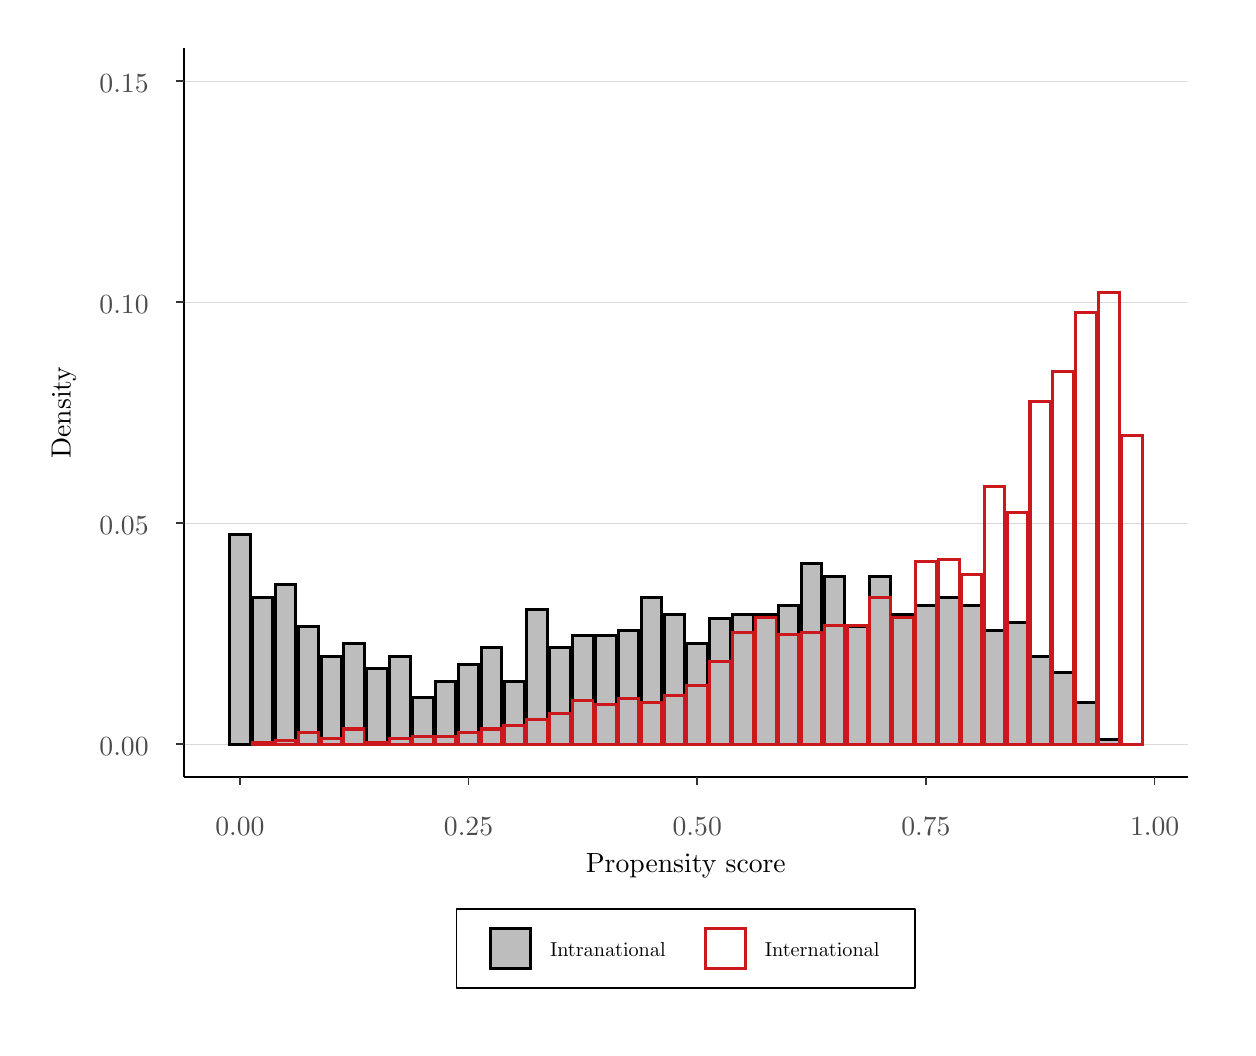
\begin{tikzpicture}[x=1pt,y=1pt]
\definecolor{fillColor}{RGB}{255,255,255}
\path[use as bounding box,fill=fillColor,fill opacity=0.00] (0,0) rectangle (433.62,361.35);
\begin{scope}
\path[clip] (  0.00,  0.00) rectangle (433.62,361.35);
\definecolor{drawColor}{RGB}{255,255,255}
\definecolor{fillColor}{RGB}{255,255,255}

\path[draw=drawColor,line width= 0.6pt,line join=round,line cap=round,fill=fillColor] ( -0.00,  0.00) rectangle (433.62,361.35);
\end{scope}
\begin{scope}
\path[clip] ( 56.47, 90.50) rectangle (419.17,354.12);
\definecolor{drawColor}{RGB}{255,255,255}

\path[draw=drawColor,line width= 0.3pt,line join=round] ( 56.47,142.42) --
	(419.17,142.42);

\path[draw=drawColor,line width= 0.3pt,line join=round] ( 56.47,222.31) --
	(419.17,222.31);

\path[draw=drawColor,line width= 0.3pt,line join=round] ( 56.47,302.20) --
	(419.17,302.20);

\path[draw=drawColor,line width= 0.3pt,line join=round] (117.99, 90.50) --
	(117.99,354.12);

\path[draw=drawColor,line width= 0.3pt,line join=round] (200.63, 90.50) --
	(200.63,354.12);

\path[draw=drawColor,line width= 0.3pt,line join=round] (283.27, 90.50) --
	(283.27,354.12);

\path[draw=drawColor,line width= 0.3pt,line join=round] (365.91, 90.50) --
	(365.91,354.12);
\definecolor{drawColor}{gray}{0.85}

\path[draw=drawColor,line width= 0.1pt,line join=round] ( 56.47,102.48) --
	(419.17,102.48);

\path[draw=drawColor,line width= 0.1pt,line join=round] ( 56.47,182.37) --
	(419.17,182.37);

\path[draw=drawColor,line width= 0.1pt,line join=round] ( 56.47,262.25) --
	(419.17,262.25);

\path[draw=drawColor,line width= 0.1pt,line join=round] ( 56.47,342.14) --
	(419.17,342.14);
\definecolor{drawColor}{RGB}{0,0,0}
\definecolor{fillColor}{gray}{0.74}

\path[draw=drawColor,line width= 1.1pt,line cap=rect,fill=fillColor] ( 72.95,102.48) rectangle ( 80.39,178.20);

\path[draw=drawColor,line width= 1.1pt,line cap=rect,fill=fillColor] ( 81.22,102.48) rectangle ( 88.65,155.49);
\definecolor{drawColor}{RGB}{203,24,29}

\path[draw=drawColor,line width= 1.1pt,line cap=rect] ( 81.22,102.48) rectangle ( 88.65,103.16);
\definecolor{drawColor}{RGB}{0,0,0}

\path[draw=drawColor,line width= 1.1pt,line cap=rect,fill=fillColor] ( 89.48,102.48) rectangle ( 96.92,160.03);
\definecolor{drawColor}{RGB}{203,24,29}

\path[draw=drawColor,line width= 1.1pt,line cap=rect] ( 89.48,102.48) rectangle ( 96.92,103.84);
\definecolor{drawColor}{RGB}{0,0,0}

\path[draw=drawColor,line width= 1.1pt,line cap=rect,fill=fillColor] ( 97.74,102.48) rectangle (105.18,144.89);
\definecolor{drawColor}{RGB}{203,24,29}

\path[draw=drawColor,line width= 1.1pt,line cap=rect] ( 97.74,102.48) rectangle (105.18,106.56);
\definecolor{drawColor}{RGB}{0,0,0}

\path[draw=drawColor,line width= 1.1pt,line cap=rect,fill=fillColor] (106.01,102.48) rectangle (113.44,134.28);
\definecolor{drawColor}{RGB}{203,24,29}

\path[draw=drawColor,line width= 1.1pt,line cap=rect] (106.01,102.48) rectangle (113.44,104.52);
\definecolor{drawColor}{RGB}{0,0,0}

\path[draw=drawColor,line width= 1.1pt,line cap=rect,fill=fillColor] (114.27,102.48) rectangle (121.71,138.83);
\definecolor{drawColor}{RGB}{203,24,29}

\path[draw=drawColor,line width= 1.1pt,line cap=rect] (114.27,102.48) rectangle (121.71,107.93);
\definecolor{drawColor}{RGB}{0,0,0}

\path[draw=drawColor,line width= 1.1pt,line cap=rect,fill=fillColor] (122.54,102.48) rectangle (129.97,129.74);
\definecolor{drawColor}{RGB}{203,24,29}

\path[draw=drawColor,line width= 1.1pt,line cap=rect] (122.54,102.48) rectangle (129.97,103.16);
\definecolor{drawColor}{RGB}{0,0,0}

\path[draw=drawColor,line width= 1.1pt,line cap=rect,fill=fillColor] (130.80,102.48) rectangle (138.24,134.28);
\definecolor{drawColor}{RGB}{203,24,29}

\path[draw=drawColor,line width= 1.1pt,line cap=rect] (130.80,102.48) rectangle (138.24,104.52);
\definecolor{drawColor}{RGB}{0,0,0}

\path[draw=drawColor,line width= 1.1pt,line cap=rect,fill=fillColor] (139.06,102.48) rectangle (146.50,119.14);
\definecolor{drawColor}{RGB}{203,24,29}

\path[draw=drawColor,line width= 1.1pt,line cap=rect] (139.06,102.48) rectangle (146.50,105.20);
\definecolor{drawColor}{RGB}{0,0,0}

\path[draw=drawColor,line width= 1.1pt,line cap=rect,fill=fillColor] (147.33,102.48) rectangle (154.76,125.20);
\definecolor{drawColor}{RGB}{203,24,29}

\path[draw=drawColor,line width= 1.1pt,line cap=rect] (147.33,102.48) rectangle (154.76,105.20);
\definecolor{drawColor}{RGB}{0,0,0}

\path[draw=drawColor,line width= 1.1pt,line cap=rect,fill=fillColor] (155.59,102.48) rectangle (163.03,131.26);
\definecolor{drawColor}{RGB}{203,24,29}

\path[draw=drawColor,line width= 1.1pt,line cap=rect] (155.59,102.48) rectangle (163.03,106.56);
\definecolor{drawColor}{RGB}{0,0,0}

\path[draw=drawColor,line width= 1.1pt,line cap=rect,fill=fillColor] (163.85,102.48) rectangle (171.29,137.31);
\definecolor{drawColor}{RGB}{203,24,29}

\path[draw=drawColor,line width= 1.1pt,line cap=rect] (163.85,102.48) rectangle (171.29,107.93);
\definecolor{drawColor}{RGB}{0,0,0}

\path[draw=drawColor,line width= 1.1pt,line cap=rect,fill=fillColor] (172.12,102.48) rectangle (179.56,125.20);
\definecolor{drawColor}{RGB}{203,24,29}

\path[draw=drawColor,line width= 1.1pt,line cap=rect] (172.12,102.48) rectangle (179.56,109.29);
\definecolor{drawColor}{RGB}{0,0,0}

\path[draw=drawColor,line width= 1.1pt,line cap=rect,fill=fillColor] (180.38,102.48) rectangle (187.82,150.94);
\definecolor{drawColor}{RGB}{203,24,29}

\path[draw=drawColor,line width= 1.1pt,line cap=rect] (180.38,102.48) rectangle (187.82,111.33);
\definecolor{drawColor}{RGB}{0,0,0}

\path[draw=drawColor,line width= 1.1pt,line cap=rect,fill=fillColor] (188.65,102.48) rectangle (196.08,137.31);
\definecolor{drawColor}{RGB}{203,24,29}

\path[draw=drawColor,line width= 1.1pt,line cap=rect] (188.65,102.48) rectangle (196.08,113.37);
\definecolor{drawColor}{RGB}{0,0,0}

\path[draw=drawColor,line width= 1.1pt,line cap=rect,fill=fillColor] (196.91,102.48) rectangle (204.35,141.86);
\definecolor{drawColor}{RGB}{203,24,29}

\path[draw=drawColor,line width= 1.1pt,line cap=rect] (196.91,102.48) rectangle (204.35,118.13);
\definecolor{drawColor}{RGB}{0,0,0}

\path[draw=drawColor,line width= 1.1pt,line cap=rect,fill=fillColor] (205.17,102.48) rectangle (212.61,141.86);
\definecolor{drawColor}{RGB}{203,24,29}

\path[draw=drawColor,line width= 1.1pt,line cap=rect] (205.17,102.48) rectangle (212.61,116.77);
\definecolor{drawColor}{RGB}{0,0,0}

\path[draw=drawColor,line width= 1.1pt,line cap=rect,fill=fillColor] (213.44,102.48) rectangle (220.87,143.37);
\definecolor{drawColor}{RGB}{203,24,29}

\path[draw=drawColor,line width= 1.1pt,line cap=rect] (213.44,102.48) rectangle (220.87,118.81);
\definecolor{drawColor}{RGB}{0,0,0}

\path[draw=drawColor,line width= 1.1pt,line cap=rect,fill=fillColor] (221.70,102.48) rectangle (229.14,155.49);
\definecolor{drawColor}{RGB}{203,24,29}

\path[draw=drawColor,line width= 1.1pt,line cap=rect] (221.70,102.48) rectangle (229.14,117.45);
\definecolor{drawColor}{RGB}{0,0,0}

\path[draw=drawColor,line width= 1.1pt,line cap=rect,fill=fillColor] (229.97,102.48) rectangle (237.40,149.43);
\definecolor{drawColor}{RGB}{203,24,29}

\path[draw=drawColor,line width= 1.1pt,line cap=rect] (229.97,102.48) rectangle (237.40,120.17);
\definecolor{drawColor}{RGB}{0,0,0}

\path[draw=drawColor,line width= 1.1pt,line cap=rect,fill=fillColor] (238.23,102.48) rectangle (245.67,138.83);
\definecolor{drawColor}{RGB}{203,24,29}

\path[draw=drawColor,line width= 1.1pt,line cap=rect] (238.23,102.48) rectangle (245.67,123.58);
\definecolor{drawColor}{RGB}{0,0,0}

\path[draw=drawColor,line width= 1.1pt,line cap=rect,fill=fillColor] (246.49,102.48) rectangle (253.93,147.91);
\definecolor{drawColor}{RGB}{203,24,29}

\path[draw=drawColor,line width= 1.1pt,line cap=rect] (246.49,102.48) rectangle (253.93,132.42);
\definecolor{drawColor}{RGB}{0,0,0}

\path[draw=drawColor,line width= 1.1pt,line cap=rect,fill=fillColor] (254.76,102.48) rectangle (262.19,149.43);
\definecolor{drawColor}{RGB}{203,24,29}

\path[draw=drawColor,line width= 1.1pt,line cap=rect] (254.76,102.48) rectangle (262.19,142.63);
\definecolor{drawColor}{RGB}{0,0,0}

\path[draw=drawColor,line width= 1.1pt,line cap=rect,fill=fillColor] (263.02,102.48) rectangle (270.46,149.43);
\definecolor{drawColor}{RGB}{203,24,29}

\path[draw=drawColor,line width= 1.1pt,line cap=rect] (263.02,102.48) rectangle (270.46,148.07);
\definecolor{drawColor}{RGB}{0,0,0}

\path[draw=drawColor,line width= 1.1pt,line cap=rect,fill=fillColor] (271.28,102.48) rectangle (278.72,152.46);
\definecolor{drawColor}{RGB}{203,24,29}

\path[draw=drawColor,line width= 1.1pt,line cap=rect] (271.28,102.48) rectangle (278.72,141.95);
\definecolor{drawColor}{RGB}{0,0,0}

\path[draw=drawColor,line width= 1.1pt,line cap=rect,fill=fillColor] (279.55,102.48) rectangle (286.99,167.60);
\definecolor{drawColor}{RGB}{203,24,29}

\path[draw=drawColor,line width= 1.1pt,line cap=rect] (279.55,102.48) rectangle (286.99,142.63);
\definecolor{drawColor}{RGB}{0,0,0}

\path[draw=drawColor,line width= 1.1pt,line cap=rect,fill=fillColor] (287.81,102.48) rectangle (295.25,163.06);
\definecolor{drawColor}{RGB}{203,24,29}

\path[draw=drawColor,line width= 1.1pt,line cap=rect] (287.81,102.48) rectangle (295.25,145.35);
\definecolor{drawColor}{RGB}{0,0,0}

\path[draw=drawColor,line width= 1.1pt,line cap=rect,fill=fillColor] (296.08,102.48) rectangle (303.51,144.89);
\definecolor{drawColor}{RGB}{203,24,29}

\path[draw=drawColor,line width= 1.1pt,line cap=rect] (296.08,102.48) rectangle (303.51,145.35);
\definecolor{drawColor}{RGB}{0,0,0}

\path[draw=drawColor,line width= 1.1pt,line cap=rect,fill=fillColor] (304.34,102.48) rectangle (311.78,163.06);
\definecolor{drawColor}{RGB}{203,24,29}

\path[draw=drawColor,line width= 1.1pt,line cap=rect] (304.34,102.48) rectangle (311.78,155.56);
\definecolor{drawColor}{RGB}{0,0,0}

\path[draw=drawColor,line width= 1.1pt,line cap=rect,fill=fillColor] (312.60,102.48) rectangle (320.04,149.43);
\definecolor{drawColor}{RGB}{203,24,29}

\path[draw=drawColor,line width= 1.1pt,line cap=rect] (312.60,102.48) rectangle (320.04,148.07);
\definecolor{drawColor}{RGB}{0,0,0}

\path[draw=drawColor,line width= 1.1pt,line cap=rect,fill=fillColor] (320.87,102.48) rectangle (328.30,152.46);
\definecolor{drawColor}{RGB}{203,24,29}

\path[draw=drawColor,line width= 1.1pt,line cap=rect] (320.87,102.48) rectangle (328.30,168.49);
\definecolor{drawColor}{RGB}{0,0,0}

\path[draw=drawColor,line width= 1.1pt,line cap=rect,fill=fillColor] (329.13,102.48) rectangle (336.57,155.49);
\definecolor{drawColor}{RGB}{203,24,29}

\path[draw=drawColor,line width= 1.1pt,line cap=rect] (329.13,102.48) rectangle (336.57,169.17);
\definecolor{drawColor}{RGB}{0,0,0}

\path[draw=drawColor,line width= 1.1pt,line cap=rect,fill=fillColor] (337.40,102.48) rectangle (344.83,152.46);
\definecolor{drawColor}{RGB}{203,24,29}

\path[draw=drawColor,line width= 1.1pt,line cap=rect] (337.40,102.48) rectangle (344.83,163.72);
\definecolor{drawColor}{RGB}{0,0,0}

\path[draw=drawColor,line width= 1.1pt,line cap=rect,fill=fillColor] (345.66,102.48) rectangle (353.10,143.37);
\definecolor{drawColor}{RGB}{203,24,29}

\path[draw=drawColor,line width= 1.1pt,line cap=rect] (345.66,102.48) rectangle (353.10,195.70);
\definecolor{drawColor}{RGB}{0,0,0}

\path[draw=drawColor,line width= 1.1pt,line cap=rect,fill=fillColor] (353.92,102.48) rectangle (361.36,146.40);
\definecolor{drawColor}{RGB}{203,24,29}

\path[draw=drawColor,line width= 1.1pt,line cap=rect] (353.92,102.48) rectangle (361.36,186.18);
\definecolor{drawColor}{RGB}{0,0,0}

\path[draw=drawColor,line width= 1.1pt,line cap=rect,fill=fillColor] (362.19,102.48) rectangle (369.62,134.28);
\definecolor{drawColor}{RGB}{203,24,29}

\path[draw=drawColor,line width= 1.1pt,line cap=rect] (362.19,102.48) rectangle (369.62,226.33);
\definecolor{drawColor}{RGB}{0,0,0}

\path[draw=drawColor,line width= 1.1pt,line cap=rect,fill=fillColor] (370.45,102.48) rectangle (377.89,128.23);
\definecolor{drawColor}{RGB}{203,24,29}

\path[draw=drawColor,line width= 1.1pt,line cap=rect] (370.45,102.48) rectangle (377.89,237.21);
\definecolor{drawColor}{RGB}{0,0,0}

\path[draw=drawColor,line width= 1.1pt,line cap=rect,fill=fillColor] (378.71,102.48) rectangle (386.15,117.63);
\definecolor{drawColor}{RGB}{203,24,29}

\path[draw=drawColor,line width= 1.1pt,line cap=rect] (378.71,102.48) rectangle (386.15,258.31);
\definecolor{drawColor}{RGB}{0,0,0}

\path[draw=drawColor,line width= 1.1pt,line cap=rect,fill=fillColor] (386.98,102.48) rectangle (394.42,104.00);
\definecolor{drawColor}{RGB}{203,24,29}

\path[draw=drawColor,line width= 1.1pt,line cap=rect] (386.98,102.48) rectangle (394.42,265.79);

\path[draw=drawColor,line width= 1.1pt,line cap=rect] (395.24,102.48) rectangle (402.68,214.08);
\end{scope}
\begin{scope}
\path[clip] (  0.00,  0.00) rectangle (433.62,361.35);
\definecolor{drawColor}{RGB}{0,0,0}

\path[draw=drawColor,line width= 0.6pt,line join=round] ( 56.47, 90.50) --
	( 56.47,354.12);
\end{scope}
\begin{scope}
\path[clip] (  0.00,  0.00) rectangle (433.62,361.35);
\definecolor{drawColor}{gray}{0.30}

\node[text=drawColor,anchor=base east,inner sep=0pt, outer sep=0pt, scale=  1.00] at ( 43.72, 98.35) {0.00};

\node[text=drawColor,anchor=base east,inner sep=0pt, outer sep=0pt, scale=  1.00] at ( 43.72,178.23) {0.05};

\node[text=drawColor,anchor=base east,inner sep=0pt, outer sep=0pt, scale=  1.00] at ( 43.72,258.12) {0.10};

\node[text=drawColor,anchor=base east,inner sep=0pt, outer sep=0pt, scale=  1.00] at ( 43.72,338.01) {0.15};
\end{scope}
\begin{scope}
\path[clip] (  0.00,  0.00) rectangle (433.62,361.35);
\definecolor{drawColor}{gray}{0.20}

\path[draw=drawColor,line width= 0.6pt,line join=round] ( 53.72,102.48) --
	( 56.47,102.48);

\path[draw=drawColor,line width= 0.6pt,line join=round] ( 53.72,182.37) --
	( 56.47,182.37);

\path[draw=drawColor,line width= 0.6pt,line join=round] ( 53.72,262.25) --
	( 56.47,262.25);

\path[draw=drawColor,line width= 0.6pt,line join=round] ( 53.72,342.14) --
	( 56.47,342.14);
\end{scope}
\begin{scope}
\path[clip] (  0.00,  0.00) rectangle (433.62,361.35);
\definecolor{drawColor}{RGB}{0,0,0}

\path[draw=drawColor,line width= 0.6pt,line join=round] ( 56.47, 90.50) --
	(419.17, 90.50);
\end{scope}
\begin{scope}
\path[clip] (  0.00,  0.00) rectangle (433.62,361.35);
\definecolor{drawColor}{gray}{0.20}

\path[draw=drawColor,line width= 0.6pt,line join=round] ( 76.67, 87.75) --
	( 76.67, 90.50);

\path[draw=drawColor,line width= 0.6pt,line join=round] (159.31, 87.75) --
	(159.31, 90.50);

\path[draw=drawColor,line width= 0.6pt,line join=round] (241.95, 87.75) --
	(241.95, 90.50);

\path[draw=drawColor,line width= 0.6pt,line join=round] (324.59, 87.75) --
	(324.59, 90.50);

\path[draw=drawColor,line width= 0.6pt,line join=round] (407.22, 87.75) --
	(407.22, 90.50);
\end{scope}
\begin{scope}
\path[clip] (  0.00,  0.00) rectangle (433.62,361.35);
\definecolor{drawColor}{gray}{0.30}

\node[text=drawColor,anchor=base,inner sep=0pt, outer sep=0pt, scale=  1.00] at ( 76.67, 69.48) {0.00};

\node[text=drawColor,anchor=base,inner sep=0pt, outer sep=0pt, scale=  1.00] at (159.31, 69.48) {0.25};

\node[text=drawColor,anchor=base,inner sep=0pt, outer sep=0pt, scale=  1.00] at (241.95, 69.48) {0.50};

\node[text=drawColor,anchor=base,inner sep=0pt, outer sep=0pt, scale=  1.00] at (324.59, 69.48) {0.75};

\node[text=drawColor,anchor=base,inner sep=0pt, outer sep=0pt, scale=  1.00] at (407.22, 69.48) {1.00};
\end{scope}
\begin{scope}
\path[clip] (  0.00,  0.00) rectangle (433.62,361.35);
\definecolor{drawColor}{RGB}{0,0,0}

\node[text=drawColor,anchor=base,inner sep=0pt, outer sep=0pt, scale=  1.00] at (237.82, 56.13) {Propensity score};
\end{scope}
\begin{scope}
\path[clip] (  0.00,  0.00) rectangle (433.62,361.35);
\definecolor{drawColor}{RGB}{0,0,0}

\node[text=drawColor,rotate= 90.00,anchor=base,inner sep=0pt, outer sep=0pt, scale=  1.00] at ( 15.49,222.31) {Density};
\end{scope}
\begin{scope}
\path[clip] (  0.00,  0.00) rectangle (433.62,361.35);
\definecolor{drawColor}{RGB}{0,0,0}
\definecolor{fillColor}{RGB}{255,255,255}

\path[draw=drawColor,line width= 0.6pt,line join=round,line cap=round,fill=fillColor] (154.91, 14.45) rectangle (320.72, 42.80);
\end{scope}
\begin{scope}
\path[clip] (  0.00,  0.00) rectangle (433.62,361.35);

\path[] (165.91, 19.95) rectangle (183.25, 37.30);
\end{scope}
\begin{scope}
\path[clip] (  0.00,  0.00) rectangle (433.62,361.35);
\definecolor{drawColor}{RGB}{0,0,0}
\definecolor{fillColor}{gray}{0.74}

\path[draw=drawColor,line width= 1.1pt,line cap=rect,fill=fillColor] (167.33, 21.38) rectangle (181.83, 35.88);
\end{scope}
\begin{scope}
\path[clip] (  0.00,  0.00) rectangle (433.62,361.35);

\path[] (243.56, 19.95) rectangle (260.90, 37.30);
\end{scope}
\begin{scope}
\path[clip] (  0.00,  0.00) rectangle (433.62,361.35);
\definecolor{drawColor}{RGB}{203,24,29}

\path[draw=drawColor,line width= 1.1pt,line cap=rect] (244.98, 21.38) rectangle (259.48, 35.88);
\end{scope}
\begin{scope}
\path[clip] (  0.00,  0.00) rectangle (433.62,361.35);
\definecolor{drawColor}{RGB}{0,0,0}

\node[text=drawColor,anchor=base west,inner sep=0pt, outer sep=0pt, scale=  0.73] at (188.75, 25.60) {Intranational};
\end{scope}
\begin{scope}
\path[clip] (  0.00,  0.00) rectangle (433.62,361.35);
\definecolor{drawColor}{RGB}{0,0,0}

\node[text=drawColor,anchor=base west,inner sep=0pt, outer sep=0pt, scale=  0.73] at (266.40, 25.60) {International};
\end{scope}
\end{tikzpicture}
}
     \end{subfigure}
     \begin{subfigure}[t]{.49\textwidth}
         \centering
         \caption{Trimmed sample}
         \label{fig: app_prop_score_trimmed}
         \scalebox{0.45}{% Created by tikzDevice version 0.12.3.1 on 2022-10-04 11:34:14
% !TEX encoding = UTF-8 Unicode
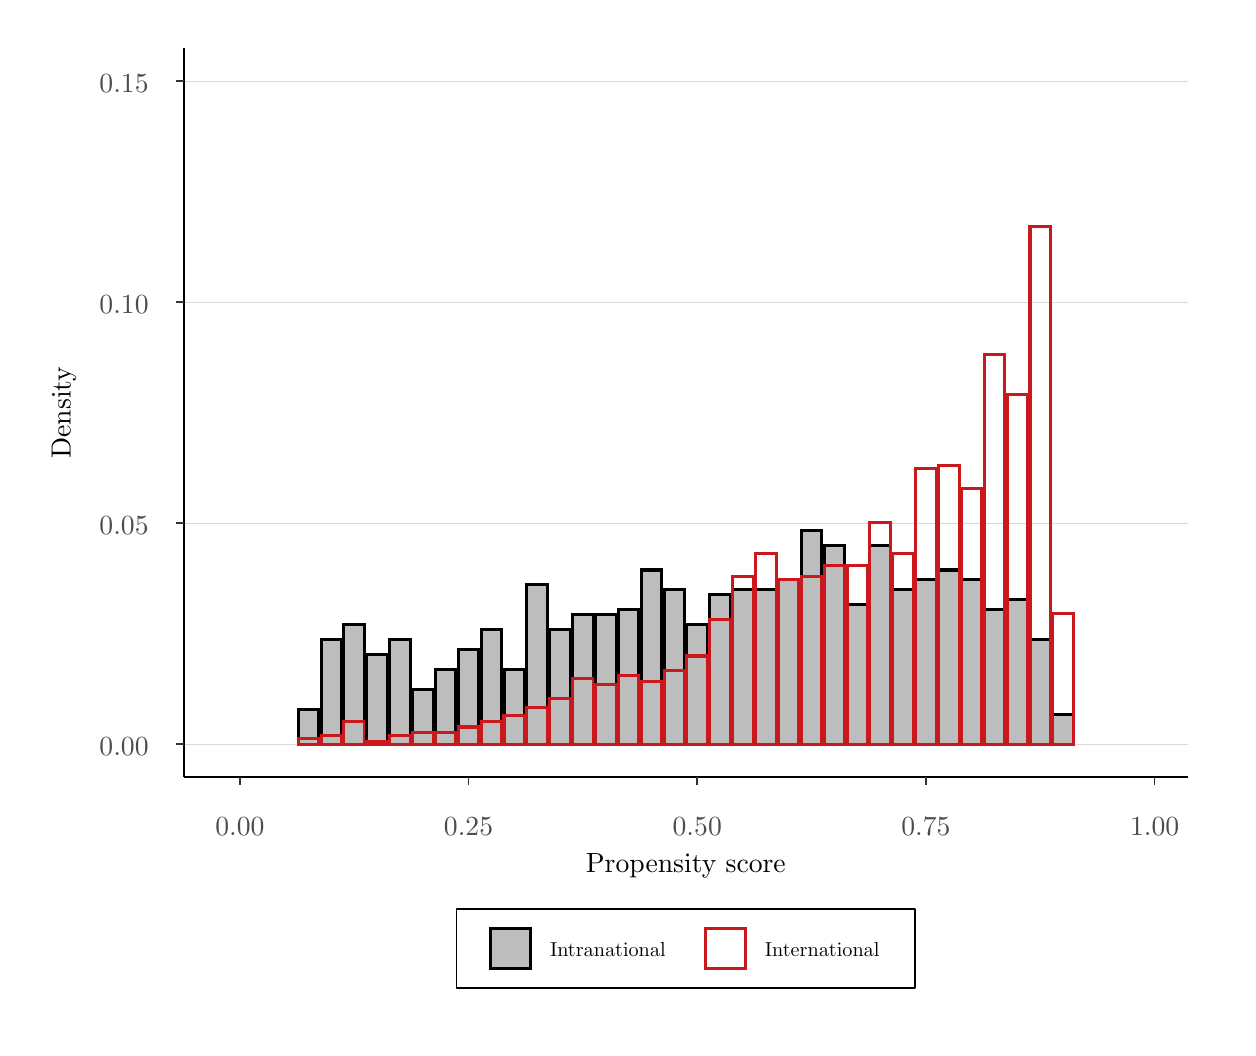
\begin{tikzpicture}[x=1pt,y=1pt]
\definecolor{fillColor}{RGB}{255,255,255}
\path[use as bounding box,fill=fillColor,fill opacity=0.00] (0,0) rectangle (433.62,361.35);
\begin{scope}
\path[clip] (  0.00,  0.00) rectangle (433.62,361.35);
\definecolor{drawColor}{RGB}{255,255,255}
\definecolor{fillColor}{RGB}{255,255,255}

\path[draw=drawColor,line width= 0.6pt,line join=round,line cap=round,fill=fillColor] ( -0.00,  0.00) rectangle (433.62,361.35);
\end{scope}
\begin{scope}
\path[clip] ( 56.47, 90.50) rectangle (419.17,354.12);
\definecolor{drawColor}{RGB}{255,255,255}

\path[draw=drawColor,line width= 0.3pt,line join=round] ( 56.47,142.42) --
	(419.17,142.42);

\path[draw=drawColor,line width= 0.3pt,line join=round] ( 56.47,222.31) --
	(419.17,222.31);

\path[draw=drawColor,line width= 0.3pt,line join=round] ( 56.47,302.20) --
	(419.17,302.20);

\path[draw=drawColor,line width= 0.3pt,line join=round] (117.99, 90.50) --
	(117.99,354.12);

\path[draw=drawColor,line width= 0.3pt,line join=round] (200.63, 90.50) --
	(200.63,354.12);

\path[draw=drawColor,line width= 0.3pt,line join=round] (283.27, 90.50) --
	(283.27,354.12);

\path[draw=drawColor,line width= 0.3pt,line join=round] (365.91, 90.50) --
	(365.91,354.12);
\definecolor{drawColor}{gray}{0.85}

\path[draw=drawColor,line width= 0.1pt,line join=round] ( 56.47,102.48) --
	(419.17,102.48);

\path[draw=drawColor,line width= 0.1pt,line join=round] ( 56.47,182.37) --
	(419.17,182.37);

\path[draw=drawColor,line width= 0.1pt,line join=round] ( 56.47,262.25) --
	(419.17,262.25);

\path[draw=drawColor,line width= 0.1pt,line join=round] ( 56.47,342.14) --
	(419.17,342.14);
\definecolor{drawColor}{RGB}{0,0,0}
\definecolor{fillColor}{gray}{0.74}

\path[draw=drawColor,line width= 1.1pt,line cap=rect,fill=fillColor] ( 97.74,102.48) rectangle (105.18,115.06);
\definecolor{drawColor}{RGB}{203,24,29}

\path[draw=drawColor,line width= 1.1pt,line cap=rect] ( 97.74,102.48) rectangle (105.18,104.53);
\definecolor{drawColor}{RGB}{0,0,0}

\path[draw=drawColor,line width= 1.1pt,line cap=rect,fill=fillColor] (106.01,102.48) rectangle (113.44,140.22);
\definecolor{drawColor}{RGB}{203,24,29}

\path[draw=drawColor,line width= 1.1pt,line cap=rect] (106.01,102.48) rectangle (113.44,105.56);
\definecolor{drawColor}{RGB}{0,0,0}

\path[draw=drawColor,line width= 1.1pt,line cap=rect,fill=fillColor] (114.27,102.48) rectangle (121.71,145.61);
\definecolor{drawColor}{RGB}{203,24,29}

\path[draw=drawColor,line width= 1.1pt,line cap=rect] (114.27,102.48) rectangle (121.71,110.70);
\definecolor{drawColor}{RGB}{0,0,0}

\path[draw=drawColor,line width= 1.1pt,line cap=rect,fill=fillColor] (122.54,102.48) rectangle (129.97,134.83);
\definecolor{drawColor}{RGB}{203,24,29}

\path[draw=drawColor,line width= 1.1pt,line cap=rect] (122.54,102.48) rectangle (129.97,103.51);
\definecolor{drawColor}{RGB}{0,0,0}

\path[draw=drawColor,line width= 1.1pt,line cap=rect,fill=fillColor] (130.80,102.48) rectangle (138.24,140.22);
\definecolor{drawColor}{RGB}{203,24,29}

\path[draw=drawColor,line width= 1.1pt,line cap=rect] (130.80,102.48) rectangle (138.24,105.56);
\definecolor{drawColor}{RGB}{0,0,0}

\path[draw=drawColor,line width= 1.1pt,line cap=rect,fill=fillColor] (139.06,102.48) rectangle (146.50,122.25);
\definecolor{drawColor}{RGB}{203,24,29}

\path[draw=drawColor,line width= 1.1pt,line cap=rect] (139.06,102.48) rectangle (146.50,106.59);
\definecolor{drawColor}{RGB}{0,0,0}

\path[draw=drawColor,line width= 1.1pt,line cap=rect,fill=fillColor] (147.33,102.48) rectangle (154.76,129.44);
\definecolor{drawColor}{RGB}{203,24,29}

\path[draw=drawColor,line width= 1.1pt,line cap=rect] (147.33,102.48) rectangle (154.76,106.59);
\definecolor{drawColor}{RGB}{0,0,0}

\path[draw=drawColor,line width= 1.1pt,line cap=rect,fill=fillColor] (155.59,102.48) rectangle (163.03,136.63);
\definecolor{drawColor}{RGB}{203,24,29}

\path[draw=drawColor,line width= 1.1pt,line cap=rect] (155.59,102.48) rectangle (163.03,108.64);
\definecolor{drawColor}{RGB}{0,0,0}

\path[draw=drawColor,line width= 1.1pt,line cap=rect,fill=fillColor] (163.85,102.48) rectangle (171.29,143.82);
\definecolor{drawColor}{RGB}{203,24,29}

\path[draw=drawColor,line width= 1.1pt,line cap=rect] (163.85,102.48) rectangle (171.29,110.70);
\definecolor{drawColor}{RGB}{0,0,0}

\path[draw=drawColor,line width= 1.1pt,line cap=rect,fill=fillColor] (172.12,102.48) rectangle (179.56,129.44);
\definecolor{drawColor}{RGB}{203,24,29}

\path[draw=drawColor,line width= 1.1pt,line cap=rect] (172.12,102.48) rectangle (179.56,112.75);
\definecolor{drawColor}{RGB}{0,0,0}

\path[draw=drawColor,line width= 1.1pt,line cap=rect,fill=fillColor] (180.38,102.48) rectangle (187.82,159.99);
\definecolor{drawColor}{RGB}{203,24,29}

\path[draw=drawColor,line width= 1.1pt,line cap=rect] (180.38,102.48) rectangle (187.82,115.83);
\definecolor{drawColor}{RGB}{0,0,0}

\path[draw=drawColor,line width= 1.1pt,line cap=rect,fill=fillColor] (188.65,102.48) rectangle (196.08,143.82);
\definecolor{drawColor}{RGB}{203,24,29}

\path[draw=drawColor,line width= 1.1pt,line cap=rect] (188.65,102.48) rectangle (196.08,118.91);
\definecolor{drawColor}{RGB}{0,0,0}

\path[draw=drawColor,line width= 1.1pt,line cap=rect,fill=fillColor] (196.91,102.48) rectangle (204.35,149.21);
\definecolor{drawColor}{RGB}{203,24,29}

\path[draw=drawColor,line width= 1.1pt,line cap=rect] (196.91,102.48) rectangle (204.35,126.10);
\definecolor{drawColor}{RGB}{0,0,0}

\path[draw=drawColor,line width= 1.1pt,line cap=rect,fill=fillColor] (205.17,102.48) rectangle (212.61,149.21);
\definecolor{drawColor}{RGB}{203,24,29}

\path[draw=drawColor,line width= 1.1pt,line cap=rect] (205.17,102.48) rectangle (212.61,124.04);
\definecolor{drawColor}{RGB}{0,0,0}

\path[draw=drawColor,line width= 1.1pt,line cap=rect,fill=fillColor] (213.44,102.48) rectangle (220.87,151.01);
\definecolor{drawColor}{RGB}{203,24,29}

\path[draw=drawColor,line width= 1.1pt,line cap=rect] (213.44,102.48) rectangle (220.87,127.12);
\definecolor{drawColor}{RGB}{0,0,0}

\path[draw=drawColor,line width= 1.1pt,line cap=rect,fill=fillColor] (221.70,102.48) rectangle (229.14,165.38);
\definecolor{drawColor}{RGB}{203,24,29}

\path[draw=drawColor,line width= 1.1pt,line cap=rect] (221.70,102.48) rectangle (229.14,125.07);
\definecolor{drawColor}{RGB}{0,0,0}

\path[draw=drawColor,line width= 1.1pt,line cap=rect,fill=fillColor] (229.97,102.48) rectangle (237.40,158.20);
\definecolor{drawColor}{RGB}{203,24,29}

\path[draw=drawColor,line width= 1.1pt,line cap=rect] (229.97,102.48) rectangle (237.40,129.18);
\definecolor{drawColor}{RGB}{0,0,0}

\path[draw=drawColor,line width= 1.1pt,line cap=rect,fill=fillColor] (238.23,102.48) rectangle (245.67,145.61);
\definecolor{drawColor}{RGB}{203,24,29}

\path[draw=drawColor,line width= 1.1pt,line cap=rect] (238.23,102.48) rectangle (245.67,134.31);
\definecolor{drawColor}{RGB}{0,0,0}

\path[draw=drawColor,line width= 1.1pt,line cap=rect,fill=fillColor] (246.49,102.48) rectangle (253.93,156.40);
\definecolor{drawColor}{RGB}{203,24,29}

\path[draw=drawColor,line width= 1.1pt,line cap=rect] (246.49,102.48) rectangle (253.93,147.66);
\definecolor{drawColor}{RGB}{0,0,0}

\path[draw=drawColor,line width= 1.1pt,line cap=rect,fill=fillColor] (254.76,102.48) rectangle (262.19,158.20);
\definecolor{drawColor}{RGB}{203,24,29}

\path[draw=drawColor,line width= 1.1pt,line cap=rect] (254.76,102.48) rectangle (262.19,163.06);
\definecolor{drawColor}{RGB}{0,0,0}

\path[draw=drawColor,line width= 1.1pt,line cap=rect,fill=fillColor] (263.02,102.48) rectangle (270.46,158.20);
\definecolor{drawColor}{RGB}{203,24,29}

\path[draw=drawColor,line width= 1.1pt,line cap=rect] (263.02,102.48) rectangle (270.46,171.28);
\definecolor{drawColor}{RGB}{0,0,0}

\path[draw=drawColor,line width= 1.1pt,line cap=rect,fill=fillColor] (271.28,102.48) rectangle (278.72,161.79);
\definecolor{drawColor}{RGB}{203,24,29}

\path[draw=drawColor,line width= 1.1pt,line cap=rect] (271.28,102.48) rectangle (278.72,162.04);
\definecolor{drawColor}{RGB}{0,0,0}

\path[draw=drawColor,line width= 1.1pt,line cap=rect,fill=fillColor] (279.55,102.48) rectangle (286.99,179.76);
\definecolor{drawColor}{RGB}{203,24,29}

\path[draw=drawColor,line width= 1.1pt,line cap=rect] (279.55,102.48) rectangle (286.99,163.06);
\definecolor{drawColor}{RGB}{0,0,0}

\path[draw=drawColor,line width= 1.1pt,line cap=rect,fill=fillColor] (287.81,102.48) rectangle (295.25,174.37);
\definecolor{drawColor}{RGB}{203,24,29}

\path[draw=drawColor,line width= 1.1pt,line cap=rect] (287.81,102.48) rectangle (295.25,167.17);
\definecolor{drawColor}{RGB}{0,0,0}

\path[draw=drawColor,line width= 1.1pt,line cap=rect,fill=fillColor] (296.08,102.48) rectangle (303.51,152.80);
\definecolor{drawColor}{RGB}{203,24,29}

\path[draw=drawColor,line width= 1.1pt,line cap=rect] (296.08,102.48) rectangle (303.51,167.17);
\definecolor{drawColor}{RGB}{0,0,0}

\path[draw=drawColor,line width= 1.1pt,line cap=rect,fill=fillColor] (304.34,102.48) rectangle (311.78,174.37);
\definecolor{drawColor}{RGB}{203,24,29}

\path[draw=drawColor,line width= 1.1pt,line cap=rect] (304.34,102.48) rectangle (311.78,182.57);
\definecolor{drawColor}{RGB}{0,0,0}

\path[draw=drawColor,line width= 1.1pt,line cap=rect,fill=fillColor] (312.60,102.48) rectangle (320.04,158.20);
\definecolor{drawColor}{RGB}{203,24,29}

\path[draw=drawColor,line width= 1.1pt,line cap=rect] (312.60,102.48) rectangle (320.04,171.28);
\definecolor{drawColor}{RGB}{0,0,0}

\path[draw=drawColor,line width= 1.1pt,line cap=rect,fill=fillColor] (320.87,102.48) rectangle (328.30,161.79);
\definecolor{drawColor}{RGB}{203,24,29}

\path[draw=drawColor,line width= 1.1pt,line cap=rect] (320.87,102.48) rectangle (328.30,202.08);
\definecolor{drawColor}{RGB}{0,0,0}

\path[draw=drawColor,line width= 1.1pt,line cap=rect,fill=fillColor] (329.13,102.48) rectangle (336.57,165.38);
\definecolor{drawColor}{RGB}{203,24,29}

\path[draw=drawColor,line width= 1.1pt,line cap=rect] (329.13,102.48) rectangle (336.57,203.11);
\definecolor{drawColor}{RGB}{0,0,0}

\path[draw=drawColor,line width= 1.1pt,line cap=rect,fill=fillColor] (337.40,102.48) rectangle (344.83,161.79);
\definecolor{drawColor}{RGB}{203,24,29}

\path[draw=drawColor,line width= 1.1pt,line cap=rect] (337.40,102.48) rectangle (344.83,194.89);
\definecolor{drawColor}{RGB}{0,0,0}

\path[draw=drawColor,line width= 1.1pt,line cap=rect,fill=fillColor] (345.66,102.48) rectangle (353.10,151.01);
\definecolor{drawColor}{RGB}{203,24,29}

\path[draw=drawColor,line width= 1.1pt,line cap=rect] (345.66,102.48) rectangle (353.10,243.16);
\definecolor{drawColor}{RGB}{0,0,0}

\path[draw=drawColor,line width= 1.1pt,line cap=rect,fill=fillColor] (353.92,102.48) rectangle (361.36,154.60);
\definecolor{drawColor}{RGB}{203,24,29}

\path[draw=drawColor,line width= 1.1pt,line cap=rect] (353.92,102.48) rectangle (361.36,228.78);
\definecolor{drawColor}{RGB}{0,0,0}

\path[draw=drawColor,line width= 1.1pt,line cap=rect,fill=fillColor] (362.19,102.48) rectangle (369.62,140.22);
\definecolor{drawColor}{RGB}{203,24,29}

\path[draw=drawColor,line width= 1.1pt,line cap=rect] (362.19,102.48) rectangle (369.62,289.36);
\definecolor{drawColor}{RGB}{0,0,0}

\path[draw=drawColor,line width= 1.1pt,line cap=rect,fill=fillColor] (370.45,102.48) rectangle (377.89,113.26);
\definecolor{drawColor}{RGB}{203,24,29}

\path[draw=drawColor,line width= 1.1pt,line cap=rect] (370.45,102.48) rectangle (377.89,149.71);
\end{scope}
\begin{scope}
\path[clip] (  0.00,  0.00) rectangle (433.62,361.35);
\definecolor{drawColor}{RGB}{0,0,0}

\path[draw=drawColor,line width= 0.6pt,line join=round] ( 56.47, 90.50) --
	( 56.47,354.12);
\end{scope}
\begin{scope}
\path[clip] (  0.00,  0.00) rectangle (433.62,361.35);
\definecolor{drawColor}{gray}{0.30}

\node[text=drawColor,anchor=base east,inner sep=0pt, outer sep=0pt, scale=  1.00] at ( 43.72, 98.35) {0.00};

\node[text=drawColor,anchor=base east,inner sep=0pt, outer sep=0pt, scale=  1.00] at ( 43.72,178.23) {0.05};

\node[text=drawColor,anchor=base east,inner sep=0pt, outer sep=0pt, scale=  1.00] at ( 43.72,258.12) {0.10};

\node[text=drawColor,anchor=base east,inner sep=0pt, outer sep=0pt, scale=  1.00] at ( 43.72,338.01) {0.15};
\end{scope}
\begin{scope}
\path[clip] (  0.00,  0.00) rectangle (433.62,361.35);
\definecolor{drawColor}{gray}{0.20}

\path[draw=drawColor,line width= 0.6pt,line join=round] ( 53.72,102.48) --
	( 56.47,102.48);

\path[draw=drawColor,line width= 0.6pt,line join=round] ( 53.72,182.37) --
	( 56.47,182.37);

\path[draw=drawColor,line width= 0.6pt,line join=round] ( 53.72,262.25) --
	( 56.47,262.25);

\path[draw=drawColor,line width= 0.6pt,line join=round] ( 53.72,342.14) --
	( 56.47,342.14);
\end{scope}
\begin{scope}
\path[clip] (  0.00,  0.00) rectangle (433.62,361.35);
\definecolor{drawColor}{RGB}{0,0,0}

\path[draw=drawColor,line width= 0.6pt,line join=round] ( 56.47, 90.50) --
	(419.17, 90.50);
\end{scope}
\begin{scope}
\path[clip] (  0.00,  0.00) rectangle (433.62,361.35);
\definecolor{drawColor}{gray}{0.20}

\path[draw=drawColor,line width= 0.6pt,line join=round] ( 76.67, 87.75) --
	( 76.67, 90.50);

\path[draw=drawColor,line width= 0.6pt,line join=round] (159.31, 87.75) --
	(159.31, 90.50);

\path[draw=drawColor,line width= 0.6pt,line join=round] (241.95, 87.75) --
	(241.95, 90.50);

\path[draw=drawColor,line width= 0.6pt,line join=round] (324.59, 87.75) --
	(324.59, 90.50);

\path[draw=drawColor,line width= 0.6pt,line join=round] (407.22, 87.75) --
	(407.22, 90.50);
\end{scope}
\begin{scope}
\path[clip] (  0.00,  0.00) rectangle (433.62,361.35);
\definecolor{drawColor}{gray}{0.30}

\node[text=drawColor,anchor=base,inner sep=0pt, outer sep=0pt, scale=  1.00] at ( 76.67, 69.48) {0.00};

\node[text=drawColor,anchor=base,inner sep=0pt, outer sep=0pt, scale=  1.00] at (159.31, 69.48) {0.25};

\node[text=drawColor,anchor=base,inner sep=0pt, outer sep=0pt, scale=  1.00] at (241.95, 69.48) {0.50};

\node[text=drawColor,anchor=base,inner sep=0pt, outer sep=0pt, scale=  1.00] at (324.59, 69.48) {0.75};

\node[text=drawColor,anchor=base,inner sep=0pt, outer sep=0pt, scale=  1.00] at (407.22, 69.48) {1.00};
\end{scope}
\begin{scope}
\path[clip] (  0.00,  0.00) rectangle (433.62,361.35);
\definecolor{drawColor}{RGB}{0,0,0}

\node[text=drawColor,anchor=base,inner sep=0pt, outer sep=0pt, scale=  1.00] at (237.82, 56.13) {Propensity score};
\end{scope}
\begin{scope}
\path[clip] (  0.00,  0.00) rectangle (433.62,361.35);
\definecolor{drawColor}{RGB}{0,0,0}

\node[text=drawColor,rotate= 90.00,anchor=base,inner sep=0pt, outer sep=0pt, scale=  1.00] at ( 15.49,222.31) {Density};
\end{scope}
\begin{scope}
\path[clip] (  0.00,  0.00) rectangle (433.62,361.35);
\definecolor{drawColor}{RGB}{0,0,0}
\definecolor{fillColor}{RGB}{255,255,255}

\path[draw=drawColor,line width= 0.6pt,line join=round,line cap=round,fill=fillColor] (154.91, 14.45) rectangle (320.72, 42.80);
\end{scope}
\begin{scope}
\path[clip] (  0.00,  0.00) rectangle (433.62,361.35);

\path[] (165.91, 19.95) rectangle (183.25, 37.30);
\end{scope}
\begin{scope}
\path[clip] (  0.00,  0.00) rectangle (433.62,361.35);
\definecolor{drawColor}{RGB}{0,0,0}
\definecolor{fillColor}{gray}{0.74}

\path[draw=drawColor,line width= 1.1pt,line cap=rect,fill=fillColor] (167.33, 21.38) rectangle (181.83, 35.88);
\end{scope}
\begin{scope}
\path[clip] (  0.00,  0.00) rectangle (433.62,361.35);

\path[] (243.56, 19.95) rectangle (260.90, 37.30);
\end{scope}
\begin{scope}
\path[clip] (  0.00,  0.00) rectangle (433.62,361.35);
\definecolor{drawColor}{RGB}{203,24,29}

\path[draw=drawColor,line width= 1.1pt,line cap=rect] (244.98, 21.38) rectangle (259.48, 35.88);
\end{scope}
\begin{scope}
\path[clip] (  0.00,  0.00) rectangle (433.62,361.35);
\definecolor{drawColor}{RGB}{0,0,0}

\node[text=drawColor,anchor=base west,inner sep=0pt, outer sep=0pt, scale=  0.73] at (188.75, 25.60) {Intranational};
\end{scope}
\begin{scope}
\path[clip] (  0.00,  0.00) rectangle (433.62,361.35);
\definecolor{drawColor}{RGB}{0,0,0}

\node[text=drawColor,anchor=base west,inner sep=0pt, outer sep=0pt, scale=  0.73] at (266.40, 25.60) {International};
\end{scope}
\end{tikzpicture}
}
     \end{subfigure}\\
     \begin{subfigure}[t]{.49\textwidth}
         \centering
         \caption{Trimmed sample - Re-estimated}
         \label{fig: app_prop_score_trimmed_re}
         \scalebox{0.45}{% Created by tikzDevice version 0.12.3.1 on 2022-10-04 11:34:14
% !TEX encoding = UTF-8 Unicode
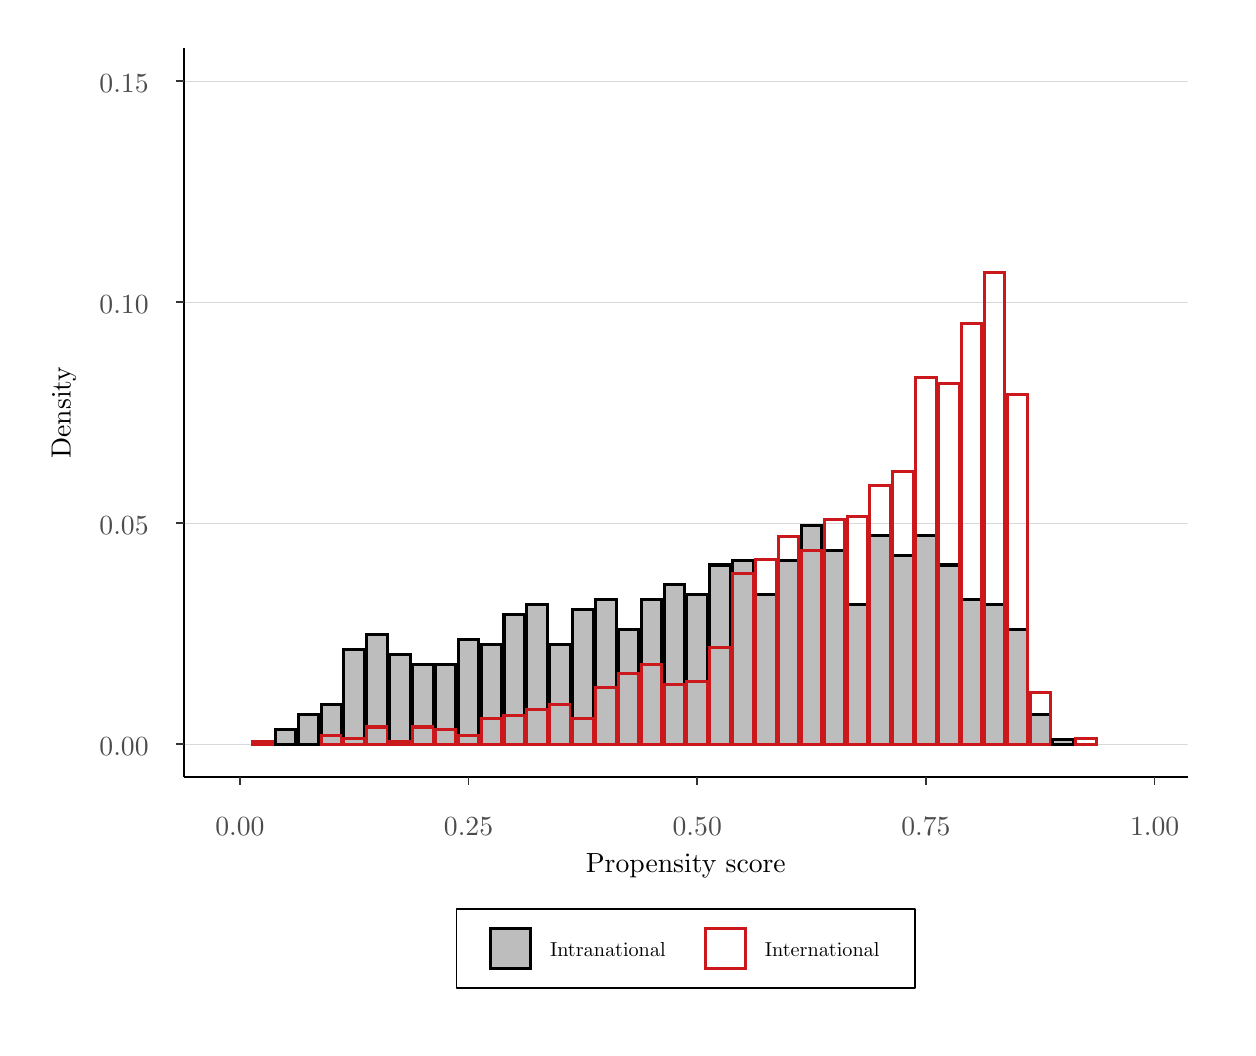
\begin{tikzpicture}[x=1pt,y=1pt]
\definecolor{fillColor}{RGB}{255,255,255}
\path[use as bounding box,fill=fillColor,fill opacity=0.00] (0,0) rectangle (433.62,361.35);
\begin{scope}
\path[clip] (  0.00,  0.00) rectangle (433.62,361.35);
\definecolor{drawColor}{RGB}{255,255,255}
\definecolor{fillColor}{RGB}{255,255,255}

\path[draw=drawColor,line width= 0.6pt,line join=round,line cap=round,fill=fillColor] ( -0.00,  0.00) rectangle (433.62,361.35);
\end{scope}
\begin{scope}
\path[clip] ( 56.47, 90.50) rectangle (419.17,354.12);
\definecolor{drawColor}{RGB}{255,255,255}

\path[draw=drawColor,line width= 0.3pt,line join=round] ( 56.47,142.42) --
	(419.17,142.42);

\path[draw=drawColor,line width= 0.3pt,line join=round] ( 56.47,222.31) --
	(419.17,222.31);

\path[draw=drawColor,line width= 0.3pt,line join=round] ( 56.47,302.20) --
	(419.17,302.20);

\path[draw=drawColor,line width= 0.3pt,line join=round] (117.99, 90.50) --
	(117.99,354.12);

\path[draw=drawColor,line width= 0.3pt,line join=round] (200.63, 90.50) --
	(200.63,354.12);

\path[draw=drawColor,line width= 0.3pt,line join=round] (283.27, 90.50) --
	(283.27,354.12);

\path[draw=drawColor,line width= 0.3pt,line join=round] (365.91, 90.50) --
	(365.91,354.12);
\definecolor{drawColor}{gray}{0.85}

\path[draw=drawColor,line width= 0.1pt,line join=round] ( 56.47,102.48) --
	(419.17,102.48);

\path[draw=drawColor,line width= 0.1pt,line join=round] ( 56.47,182.37) --
	(419.17,182.37);

\path[draw=drawColor,line width= 0.1pt,line join=round] ( 56.47,262.25) --
	(419.17,262.25);

\path[draw=drawColor,line width= 0.1pt,line join=round] ( 56.47,342.14) --
	(419.17,342.14);
\definecolor{drawColor}{RGB}{203,24,29}

\path[draw=drawColor,line width= 1.1pt,line cap=rect] ( 81.22,102.48) rectangle ( 88.65,103.51);
\definecolor{drawColor}{RGB}{0,0,0}
\definecolor{fillColor}{gray}{0.74}

\path[draw=drawColor,line width= 1.1pt,line cap=rect,fill=fillColor] ( 89.48,102.48) rectangle ( 96.92,107.87);

\path[draw=drawColor,line width= 1.1pt,line cap=rect,fill=fillColor] ( 97.74,102.48) rectangle (105.18,113.26);

\path[draw=drawColor,line width= 1.1pt,line cap=rect,fill=fillColor] (106.01,102.48) rectangle (113.44,116.86);
\definecolor{drawColor}{RGB}{203,24,29}

\path[draw=drawColor,line width= 1.1pt,line cap=rect] (106.01,102.48) rectangle (113.44,105.56);
\definecolor{drawColor}{RGB}{0,0,0}

\path[draw=drawColor,line width= 1.1pt,line cap=rect,fill=fillColor] (114.27,102.48) rectangle (121.71,136.63);
\definecolor{drawColor}{RGB}{203,24,29}

\path[draw=drawColor,line width= 1.1pt,line cap=rect] (114.27,102.48) rectangle (121.71,104.53);
\definecolor{drawColor}{RGB}{0,0,0}

\path[draw=drawColor,line width= 1.1pt,line cap=rect,fill=fillColor] (122.54,102.48) rectangle (129.97,142.02);
\definecolor{drawColor}{RGB}{203,24,29}

\path[draw=drawColor,line width= 1.1pt,line cap=rect] (122.54,102.48) rectangle (129.97,108.64);
\definecolor{drawColor}{RGB}{0,0,0}

\path[draw=drawColor,line width= 1.1pt,line cap=rect,fill=fillColor] (130.80,102.48) rectangle (138.24,134.83);
\definecolor{drawColor}{RGB}{203,24,29}

\path[draw=drawColor,line width= 1.1pt,line cap=rect] (130.80,102.48) rectangle (138.24,103.51);
\definecolor{drawColor}{RGB}{0,0,0}

\path[draw=drawColor,line width= 1.1pt,line cap=rect,fill=fillColor] (139.06,102.48) rectangle (146.50,131.24);
\definecolor{drawColor}{RGB}{203,24,29}

\path[draw=drawColor,line width= 1.1pt,line cap=rect] (139.06,102.48) rectangle (146.50,108.64);
\definecolor{drawColor}{RGB}{0,0,0}

\path[draw=drawColor,line width= 1.1pt,line cap=rect,fill=fillColor] (147.33,102.48) rectangle (154.76,131.24);
\definecolor{drawColor}{RGB}{203,24,29}

\path[draw=drawColor,line width= 1.1pt,line cap=rect] (147.33,102.48) rectangle (154.76,107.62);
\definecolor{drawColor}{RGB}{0,0,0}

\path[draw=drawColor,line width= 1.1pt,line cap=rect,fill=fillColor] (155.59,102.48) rectangle (163.03,140.22);
\definecolor{drawColor}{RGB}{203,24,29}

\path[draw=drawColor,line width= 1.1pt,line cap=rect] (155.59,102.48) rectangle (163.03,105.56);
\definecolor{drawColor}{RGB}{0,0,0}

\path[draw=drawColor,line width= 1.1pt,line cap=rect,fill=fillColor] (163.85,102.48) rectangle (171.29,138.43);
\definecolor{drawColor}{RGB}{203,24,29}

\path[draw=drawColor,line width= 1.1pt,line cap=rect] (163.85,102.48) rectangle (171.29,111.72);
\definecolor{drawColor}{RGB}{0,0,0}

\path[draw=drawColor,line width= 1.1pt,line cap=rect,fill=fillColor] (172.12,102.48) rectangle (179.56,149.21);
\definecolor{drawColor}{RGB}{203,24,29}

\path[draw=drawColor,line width= 1.1pt,line cap=rect] (172.12,102.48) rectangle (179.56,112.75);
\definecolor{drawColor}{RGB}{0,0,0}

\path[draw=drawColor,line width= 1.1pt,line cap=rect,fill=fillColor] (180.38,102.48) rectangle (187.82,152.80);
\definecolor{drawColor}{RGB}{203,24,29}

\path[draw=drawColor,line width= 1.1pt,line cap=rect] (180.38,102.48) rectangle (187.82,114.80);
\definecolor{drawColor}{RGB}{0,0,0}

\path[draw=drawColor,line width= 1.1pt,line cap=rect,fill=fillColor] (188.65,102.48) rectangle (196.08,138.43);
\definecolor{drawColor}{RGB}{203,24,29}

\path[draw=drawColor,line width= 1.1pt,line cap=rect] (188.65,102.48) rectangle (196.08,116.86);
\definecolor{drawColor}{RGB}{0,0,0}

\path[draw=drawColor,line width= 1.1pt,line cap=rect,fill=fillColor] (196.91,102.48) rectangle (204.35,151.01);
\definecolor{drawColor}{RGB}{203,24,29}

\path[draw=drawColor,line width= 1.1pt,line cap=rect] (196.91,102.48) rectangle (204.35,111.72);
\definecolor{drawColor}{RGB}{0,0,0}

\path[draw=drawColor,line width= 1.1pt,line cap=rect,fill=fillColor] (205.17,102.48) rectangle (212.61,154.60);
\definecolor{drawColor}{RGB}{203,24,29}

\path[draw=drawColor,line width= 1.1pt,line cap=rect] (205.17,102.48) rectangle (212.61,123.02);
\definecolor{drawColor}{RGB}{0,0,0}

\path[draw=drawColor,line width= 1.1pt,line cap=rect,fill=fillColor] (213.44,102.48) rectangle (220.87,143.82);
\definecolor{drawColor}{RGB}{203,24,29}

\path[draw=drawColor,line width= 1.1pt,line cap=rect] (213.44,102.48) rectangle (220.87,128.15);
\definecolor{drawColor}{RGB}{0,0,0}

\path[draw=drawColor,line width= 1.1pt,line cap=rect,fill=fillColor] (221.70,102.48) rectangle (229.14,154.60);
\definecolor{drawColor}{RGB}{203,24,29}

\path[draw=drawColor,line width= 1.1pt,line cap=rect] (221.70,102.48) rectangle (229.14,131.23);
\definecolor{drawColor}{RGB}{0,0,0}

\path[draw=drawColor,line width= 1.1pt,line cap=rect,fill=fillColor] (229.97,102.48) rectangle (237.40,159.99);
\definecolor{drawColor}{RGB}{203,24,29}

\path[draw=drawColor,line width= 1.1pt,line cap=rect] (229.97,102.48) rectangle (237.40,124.04);
\definecolor{drawColor}{RGB}{0,0,0}

\path[draw=drawColor,line width= 1.1pt,line cap=rect,fill=fillColor] (238.23,102.48) rectangle (245.67,156.40);
\definecolor{drawColor}{RGB}{203,24,29}

\path[draw=drawColor,line width= 1.1pt,line cap=rect] (238.23,102.48) rectangle (245.67,125.07);
\definecolor{drawColor}{RGB}{0,0,0}

\path[draw=drawColor,line width= 1.1pt,line cap=rect,fill=fillColor] (246.49,102.48) rectangle (253.93,167.18);
\definecolor{drawColor}{RGB}{203,24,29}

\path[draw=drawColor,line width= 1.1pt,line cap=rect] (246.49,102.48) rectangle (253.93,137.39);
\definecolor{drawColor}{RGB}{0,0,0}

\path[draw=drawColor,line width= 1.1pt,line cap=rect,fill=fillColor] (254.76,102.48) rectangle (262.19,168.98);
\definecolor{drawColor}{RGB}{203,24,29}

\path[draw=drawColor,line width= 1.1pt,line cap=rect] (254.76,102.48) rectangle (262.19,164.09);
\definecolor{drawColor}{RGB}{0,0,0}

\path[draw=drawColor,line width= 1.1pt,line cap=rect,fill=fillColor] (263.02,102.48) rectangle (270.46,156.40);
\definecolor{drawColor}{RGB}{203,24,29}

\path[draw=drawColor,line width= 1.1pt,line cap=rect] (263.02,102.48) rectangle (270.46,169.22);
\definecolor{drawColor}{RGB}{0,0,0}

\path[draw=drawColor,line width= 1.1pt,line cap=rect,fill=fillColor] (271.28,102.48) rectangle (278.72,168.98);
\definecolor{drawColor}{RGB}{203,24,29}

\path[draw=drawColor,line width= 1.1pt,line cap=rect] (271.28,102.48) rectangle (278.72,177.44);
\definecolor{drawColor}{RGB}{0,0,0}

\path[draw=drawColor,line width= 1.1pt,line cap=rect,fill=fillColor] (279.55,102.48) rectangle (286.99,181.56);
\definecolor{drawColor}{RGB}{203,24,29}

\path[draw=drawColor,line width= 1.1pt,line cap=rect] (279.55,102.48) rectangle (286.99,172.30);
\definecolor{drawColor}{RGB}{0,0,0}

\path[draw=drawColor,line width= 1.1pt,line cap=rect,fill=fillColor] (287.81,102.48) rectangle (295.25,172.57);
\definecolor{drawColor}{RGB}{203,24,29}

\path[draw=drawColor,line width= 1.1pt,line cap=rect] (287.81,102.48) rectangle (295.25,183.60);
\definecolor{drawColor}{RGB}{0,0,0}

\path[draw=drawColor,line width= 1.1pt,line cap=rect,fill=fillColor] (296.08,102.48) rectangle (303.51,152.80);
\definecolor{drawColor}{RGB}{203,24,29}

\path[draw=drawColor,line width= 1.1pt,line cap=rect] (296.08,102.48) rectangle (303.51,184.63);
\definecolor{drawColor}{RGB}{0,0,0}

\path[draw=drawColor,line width= 1.1pt,line cap=rect,fill=fillColor] (304.34,102.48) rectangle (311.78,177.96);
\definecolor{drawColor}{RGB}{203,24,29}

\path[draw=drawColor,line width= 1.1pt,line cap=rect] (304.34,102.48) rectangle (311.78,195.92);
\definecolor{drawColor}{RGB}{0,0,0}

\path[draw=drawColor,line width= 1.1pt,line cap=rect,fill=fillColor] (312.60,102.48) rectangle (320.04,170.78);
\definecolor{drawColor}{RGB}{203,24,29}

\path[draw=drawColor,line width= 1.1pt,line cap=rect] (312.60,102.48) rectangle (320.04,201.06);
\definecolor{drawColor}{RGB}{0,0,0}

\path[draw=drawColor,line width= 1.1pt,line cap=rect,fill=fillColor] (320.87,102.48) rectangle (328.30,177.96);
\definecolor{drawColor}{RGB}{203,24,29}

\path[draw=drawColor,line width= 1.1pt,line cap=rect] (320.87,102.48) rectangle (328.30,234.94);
\definecolor{drawColor}{RGB}{0,0,0}

\path[draw=drawColor,line width= 1.1pt,line cap=rect,fill=fillColor] (329.13,102.48) rectangle (336.57,167.18);
\definecolor{drawColor}{RGB}{203,24,29}

\path[draw=drawColor,line width= 1.1pt,line cap=rect] (329.13,102.48) rectangle (336.57,232.89);
\definecolor{drawColor}{RGB}{0,0,0}

\path[draw=drawColor,line width= 1.1pt,line cap=rect,fill=fillColor] (337.40,102.48) rectangle (344.83,154.60);
\definecolor{drawColor}{RGB}{203,24,29}

\path[draw=drawColor,line width= 1.1pt,line cap=rect] (337.40,102.48) rectangle (344.83,254.45);
\definecolor{drawColor}{RGB}{0,0,0}

\path[draw=drawColor,line width= 1.1pt,line cap=rect,fill=fillColor] (345.66,102.48) rectangle (353.10,152.80);
\definecolor{drawColor}{RGB}{203,24,29}

\path[draw=drawColor,line width= 1.1pt,line cap=rect] (345.66,102.48) rectangle (353.10,272.93);
\definecolor{drawColor}{RGB}{0,0,0}

\path[draw=drawColor,line width= 1.1pt,line cap=rect,fill=fillColor] (353.92,102.48) rectangle (361.36,143.82);
\definecolor{drawColor}{RGB}{203,24,29}

\path[draw=drawColor,line width= 1.1pt,line cap=rect] (353.92,102.48) rectangle (361.36,228.78);
\definecolor{drawColor}{RGB}{0,0,0}

\path[draw=drawColor,line width= 1.1pt,line cap=rect,fill=fillColor] (362.19,102.48) rectangle (369.62,113.26);
\definecolor{drawColor}{RGB}{203,24,29}

\path[draw=drawColor,line width= 1.1pt,line cap=rect] (362.19,102.48) rectangle (369.62,120.96);
\definecolor{drawColor}{RGB}{0,0,0}

\path[draw=drawColor,line width= 1.1pt,line cap=rect,fill=fillColor] (370.45,102.48) rectangle (377.89,104.28);
\definecolor{drawColor}{RGB}{203,24,29}

\path[draw=drawColor,line width= 1.1pt,line cap=rect] (378.71,102.48) rectangle (386.15,104.53);
\end{scope}
\begin{scope}
\path[clip] (  0.00,  0.00) rectangle (433.62,361.35);
\definecolor{drawColor}{RGB}{0,0,0}

\path[draw=drawColor,line width= 0.6pt,line join=round] ( 56.47, 90.50) --
	( 56.47,354.12);
\end{scope}
\begin{scope}
\path[clip] (  0.00,  0.00) rectangle (433.62,361.35);
\definecolor{drawColor}{gray}{0.30}

\node[text=drawColor,anchor=base east,inner sep=0pt, outer sep=0pt, scale=  1.00] at ( 43.72, 98.35) {0.00};

\node[text=drawColor,anchor=base east,inner sep=0pt, outer sep=0pt, scale=  1.00] at ( 43.72,178.23) {0.05};

\node[text=drawColor,anchor=base east,inner sep=0pt, outer sep=0pt, scale=  1.00] at ( 43.72,258.12) {0.10};

\node[text=drawColor,anchor=base east,inner sep=0pt, outer sep=0pt, scale=  1.00] at ( 43.72,338.01) {0.15};
\end{scope}
\begin{scope}
\path[clip] (  0.00,  0.00) rectangle (433.62,361.35);
\definecolor{drawColor}{gray}{0.20}

\path[draw=drawColor,line width= 0.6pt,line join=round] ( 53.72,102.48) --
	( 56.47,102.48);

\path[draw=drawColor,line width= 0.6pt,line join=round] ( 53.72,182.37) --
	( 56.47,182.37);

\path[draw=drawColor,line width= 0.6pt,line join=round] ( 53.72,262.25) --
	( 56.47,262.25);

\path[draw=drawColor,line width= 0.6pt,line join=round] ( 53.72,342.14) --
	( 56.47,342.14);
\end{scope}
\begin{scope}
\path[clip] (  0.00,  0.00) rectangle (433.62,361.35);
\definecolor{drawColor}{RGB}{0,0,0}

\path[draw=drawColor,line width= 0.6pt,line join=round] ( 56.47, 90.50) --
	(419.17, 90.50);
\end{scope}
\begin{scope}
\path[clip] (  0.00,  0.00) rectangle (433.62,361.35);
\definecolor{drawColor}{gray}{0.20}

\path[draw=drawColor,line width= 0.6pt,line join=round] ( 76.67, 87.75) --
	( 76.67, 90.50);

\path[draw=drawColor,line width= 0.6pt,line join=round] (159.31, 87.75) --
	(159.31, 90.50);

\path[draw=drawColor,line width= 0.6pt,line join=round] (241.95, 87.75) --
	(241.95, 90.50);

\path[draw=drawColor,line width= 0.6pt,line join=round] (324.59, 87.75) --
	(324.59, 90.50);

\path[draw=drawColor,line width= 0.6pt,line join=round] (407.22, 87.75) --
	(407.22, 90.50);
\end{scope}
\begin{scope}
\path[clip] (  0.00,  0.00) rectangle (433.62,361.35);
\definecolor{drawColor}{gray}{0.30}

\node[text=drawColor,anchor=base,inner sep=0pt, outer sep=0pt, scale=  1.00] at ( 76.67, 69.48) {0.00};

\node[text=drawColor,anchor=base,inner sep=0pt, outer sep=0pt, scale=  1.00] at (159.31, 69.48) {0.25};

\node[text=drawColor,anchor=base,inner sep=0pt, outer sep=0pt, scale=  1.00] at (241.95, 69.48) {0.50};

\node[text=drawColor,anchor=base,inner sep=0pt, outer sep=0pt, scale=  1.00] at (324.59, 69.48) {0.75};

\node[text=drawColor,anchor=base,inner sep=0pt, outer sep=0pt, scale=  1.00] at (407.22, 69.48) {1.00};
\end{scope}
\begin{scope}
\path[clip] (  0.00,  0.00) rectangle (433.62,361.35);
\definecolor{drawColor}{RGB}{0,0,0}

\node[text=drawColor,anchor=base,inner sep=0pt, outer sep=0pt, scale=  1.00] at (237.82, 56.13) {Propensity score};
\end{scope}
\begin{scope}
\path[clip] (  0.00,  0.00) rectangle (433.62,361.35);
\definecolor{drawColor}{RGB}{0,0,0}

\node[text=drawColor,rotate= 90.00,anchor=base,inner sep=0pt, outer sep=0pt, scale=  1.00] at ( 15.49,222.31) {Density};
\end{scope}
\begin{scope}
\path[clip] (  0.00,  0.00) rectangle (433.62,361.35);
\definecolor{drawColor}{RGB}{0,0,0}
\definecolor{fillColor}{RGB}{255,255,255}

\path[draw=drawColor,line width= 0.6pt,line join=round,line cap=round,fill=fillColor] (154.91, 14.45) rectangle (320.72, 42.80);
\end{scope}
\begin{scope}
\path[clip] (  0.00,  0.00) rectangle (433.62,361.35);

\path[] (165.91, 19.95) rectangle (183.25, 37.30);
\end{scope}
\begin{scope}
\path[clip] (  0.00,  0.00) rectangle (433.62,361.35);
\definecolor{drawColor}{RGB}{0,0,0}
\definecolor{fillColor}{gray}{0.74}

\path[draw=drawColor,line width= 1.1pt,line cap=rect,fill=fillColor] (167.33, 21.38) rectangle (181.83, 35.88);
\end{scope}
\begin{scope}
\path[clip] (  0.00,  0.00) rectangle (433.62,361.35);

\path[] (243.56, 19.95) rectangle (260.90, 37.30);
\end{scope}
\begin{scope}
\path[clip] (  0.00,  0.00) rectangle (433.62,361.35);
\definecolor{drawColor}{RGB}{203,24,29}

\path[draw=drawColor,line width= 1.1pt,line cap=rect] (244.98, 21.38) rectangle (259.48, 35.88);
\end{scope}
\begin{scope}
\path[clip] (  0.00,  0.00) rectangle (433.62,361.35);
\definecolor{drawColor}{RGB}{0,0,0}

\node[text=drawColor,anchor=base west,inner sep=0pt, outer sep=0pt, scale=  0.73] at (188.75, 25.60) {Intranational};
\end{scope}
\begin{scope}
\path[clip] (  0.00,  0.00) rectangle (433.62,361.35);
\definecolor{drawColor}{RGB}{0,0,0}

\node[text=drawColor,anchor=base west,inner sep=0pt, outer sep=0pt, scale=  0.73] at (266.40, 25.60) {International};
\end{scope}
\end{tikzpicture}
}
     \end{subfigure}
     \parbox{\textwidth}{
        \begin{spacing}{1} 
            {\footnotesize 
            \textit{Notes}: These figures provide the conditional distributions of predicted propensity scores based on the augmented model. We plot the conditional distribution of national pairs in grey and the one for international pairs in red. Panel (a) and (b) show the distributions for the full and trimmed sample respectively. Panel (c) plots the conditional distributions of predicted propensity scores for the trimmed sample after re-estimating the augmented model on the trimmed sample.}
        \end{spacing}}
 \end{figure} 



\begin{figure}[H]
    \centering
    \caption{Trimming cut-off: Grid search results}
    \label{fig: app_prop_score_trimming_algo}
    \scalebox{0.85}{% Created by tikzDevice version 0.12.3.1 on 2022-10-04 11:33:44
% !TEX encoding = UTF-8 Unicode
\begin{tikzpicture}[x=1pt,y=1pt]
\definecolor{fillColor}{RGB}{255,255,255}
\path[use as bounding box,fill=fillColor,fill opacity=0.00] (0,0) rectangle (433.62,361.35);
\begin{scope}
\path[clip] (  0.00,  0.00) rectangle (433.62,361.35);
\definecolor{drawColor}{RGB}{255,255,255}
\definecolor{fillColor}{RGB}{255,255,255}

\path[draw=drawColor,line width= 0.6pt,line join=round,line cap=round,fill=fillColor] ( -0.00,  0.00) rectangle (433.62,361.35);
\end{scope}
\begin{scope}
\path[clip] ( 51.24, 90.50) rectangle (419.17,354.12);
\definecolor{drawColor}{RGB}{255,255,255}

\path[draw=drawColor,line width= 0.3pt,line join=round] ( 51.24,122.45) --
	(419.17,122.45);

\path[draw=drawColor,line width= 0.3pt,line join=round] ( 51.24,162.40) --
	(419.17,162.40);

\path[draw=drawColor,line width= 0.3pt,line join=round] ( 51.24,202.34) --
	(419.17,202.34);

\path[draw=drawColor,line width= 0.3pt,line join=round] ( 51.24,242.28) --
	(419.17,242.28);

\path[draw=drawColor,line width= 0.3pt,line join=round] ( 51.24,282.23) --
	(419.17,282.23);

\path[draw=drawColor,line width= 0.3pt,line join=round] ( 51.24,322.17) --
	(419.17,322.17);

\path[draw=drawColor,line width= 0.3pt,line join=round] ( 84.72, 90.50) --
	( 84.72,354.12);

\path[draw=drawColor,line width= 0.3pt,line join=round] (118.24, 90.50) --
	(118.24,354.12);

\path[draw=drawColor,line width= 0.3pt,line join=round] (151.75, 90.50) --
	(151.75,354.12);

\path[draw=drawColor,line width= 0.3pt,line join=round] (185.27, 90.50) --
	(185.27,354.12);

\path[draw=drawColor,line width= 0.3pt,line join=round] (218.78, 90.50) --
	(218.78,354.12);

\path[draw=drawColor,line width= 0.3pt,line join=round] (252.30, 90.50) --
	(252.30,354.12);

\path[draw=drawColor,line width= 0.3pt,line join=round] (285.81, 90.50) --
	(285.81,354.12);

\path[draw=drawColor,line width= 0.3pt,line join=round] (319.33, 90.50) --
	(319.33,354.12);

\path[draw=drawColor,line width= 0.3pt,line join=round] (352.84, 90.50) --
	(352.84,354.12);

\path[draw=drawColor,line width= 0.3pt,line join=round] (386.36, 90.50) --
	(386.36,354.12);
\definecolor{drawColor}{gray}{0.85}

\path[draw=drawColor,line width= 0.1pt,line join=round] ( 51.24,102.48) --
	(419.17,102.48);

\path[draw=drawColor,line width= 0.1pt,line join=round] ( 51.24,142.42) --
	(419.17,142.42);

\path[draw=drawColor,line width= 0.1pt,line join=round] ( 51.24,182.37) --
	(419.17,182.37);

\path[draw=drawColor,line width= 0.1pt,line join=round] ( 51.24,222.31) --
	(419.17,222.31);

\path[draw=drawColor,line width= 0.1pt,line join=round] ( 51.24,262.25) --
	(419.17,262.25);

\path[draw=drawColor,line width= 0.1pt,line join=round] ( 51.24,302.20) --
	(419.17,302.20);

\path[draw=drawColor,line width= 0.1pt,line join=round] ( 51.24,342.14) --
	(419.17,342.14);
\definecolor{drawColor}{RGB}{0,0,0}

\path[draw=drawColor,line width= 0.6pt,line join=round] ( 67.97,330.74) --
	( 68.64,277.25) --
	( 69.31,271.50) --
	( 69.98,268.06) --
	( 70.65,265.55) --
	( 71.32,263.55) --
	( 71.99,261.89) --
	( 72.66,260.46) --
	( 73.33,259.20) --
	( 74.00,258.07) --
	( 74.67,257.04) --
	( 75.34,256.11) --
	( 76.01,255.22) --
	( 76.68,254.41) --
	( 77.35,253.64) --
	( 78.02,252.90) --
	( 78.69,252.19) --
	( 79.36,251.53) --
	( 80.03,250.89) --
	( 80.70,250.27) --
	( 81.37,249.69) --
	( 82.04,249.10) --
	( 82.71,248.55) --
	( 83.38,248.00) --
	( 84.05,247.50) --
	( 84.72,247.01) --
	( 85.39,246.51) --
	( 86.07,246.04) --
	( 86.74,245.58) --
	( 87.41,245.12) --
	( 88.08,244.66) --
	( 88.75,244.20) --
	( 89.42,243.79) --
	( 90.09,243.38) --
	( 90.76,242.97) --
	( 91.43,242.53) --
	( 92.10,242.15) --
	( 92.77,241.76) --
	( 93.44,241.35) --
	( 94.11,240.95) --
	( 94.78,240.54) --
	( 95.45,240.13) --
	( 96.12,239.75) --
	( 96.79,239.38) --
	( 97.46,239.04) --
	( 98.13,238.68) --
	( 98.80,238.34) --
	( 99.47,237.97) --
	(100.14,237.63) --
	(100.81,237.28) --
	(101.48,236.94) --
	(102.15,236.60) --
	(102.82,236.27) --
	(103.49,235.90) --
	(104.16,235.58) --
	(104.83,235.21) --
	(105.50,234.87) --
	(106.17,234.54) --
	(106.84,234.17) --
	(107.51,233.92) --
	(108.18,233.54) --
	(108.85,233.20) --
	(109.53,232.87) --
	(110.20,232.48) --
	(110.87,232.14) --
	(111.54,231.83) --
	(112.21,231.49) --
	(112.88,231.15) --
	(113.55,230.82) --
	(114.22,230.55) --
	(114.89,230.15) --
	(115.56,229.89) --
	(116.23,229.59) --
	(116.90,229.26) --
	(117.57,228.95) --
	(118.24,228.63) --
	(118.91,228.32) --
	(119.58,227.93) --
	(120.25,227.57) --
	(120.92,227.19) --
	(121.59,226.87) --
	(122.26,226.48) --
	(122.93,226.14) --
	(123.60,225.66) --
	(124.27,225.32) --
	(124.94,224.95) --
	(125.61,224.53) --
	(126.28,224.08) --
	(126.95,223.79) --
	(127.62,223.68) --
	(128.29,223.25) --
	(128.96,223.21) --
	(129.63,222.79) --
	(130.30,222.34) --
	(130.97,221.99) --
	(131.64,221.46) --
	(132.32,221.03) --
	(132.99,220.60) --
	(133.66,220.19) --
	(134.33,219.60) --
	(135.00,219.24) --
	(135.67,218.81) --
	(136.34,218.50) --
	(137.01,218.06) --
	(137.68,217.52) --
	(138.35,216.92) --
	(139.02,216.49) --
	(139.69,216.01) --
	(140.36,215.34) --
	(141.03,214.63) --
	(141.70,213.95) --
	(142.37,213.30) --
	(143.04,212.38) --
	(143.71,211.64) --
	(144.38,210.46) --
	(145.05,209.58) --
	(145.72,208.88) --
	(146.39,209.04) --
	(147.06,207.41) --
	(147.73,205.59) --
	(148.40,204.21) --
	(149.07,203.12) --
	(149.74,201.94) --
	(150.41,200.96) --
	(151.08,199.92) --
	(151.75,195.31) --
	(152.42,193.43);

\path[draw=drawColor,line width= 0.6pt,line join=round] (293.18,165.86) --
	(293.86,181.07) --
	(294.53,186.00) --
	(295.20,188.33) --
	(295.87,191.24) --
	(296.54,192.96) --
	(297.21,193.67) --
	(297.88,195.60) --
	(298.55,196.12) --
	(299.22,197.11) --
	(299.89,198.82) --
	(300.56,199.37) --
	(301.23,200.05) --
	(301.90,201.13) --
	(302.57,201.95) --
	(303.24,202.33) --
	(303.91,203.27) --
	(304.58,204.02) --
	(305.25,204.41) --
	(305.92,205.24) --
	(306.59,205.49) --
	(307.26,206.06) --
	(307.93,206.38) --
	(308.60,206.68) --
	(309.27,207.17) --
	(309.94,207.31) --
	(310.61,207.39) --
	(311.28,207.84) --
	(311.95,208.03) --
	(312.62,208.22) --
	(313.29,208.35) --
	(313.96,208.53) --
	(314.63,208.93) --
	(315.30,209.36) --
	(315.97,209.52) --
	(316.65,209.73) --
	(317.32,209.93) --
	(317.99,210.18) --
	(318.66,210.42) --
	(319.33,210.56) --
	(320.00,210.79) --
	(320.67,210.93) --
	(321.34,211.38) --
	(322.01,211.63) --
	(322.68,211.86) --
	(323.35,212.02) --
	(324.02,212.11) --
	(324.69,212.23) --
	(325.36,212.42) --
	(326.03,212.46) --
	(326.70,212.68) --
	(327.37,212.79) --
	(328.04,213.00) --
	(328.71,213.17) --
	(329.38,213.37) --
	(330.05,213.50) --
	(330.72,213.72) --
	(331.39,213.82) --
	(332.06,213.95) --
	(332.73,214.10) --
	(333.40,214.19) --
	(334.07,214.37) --
	(334.74,214.46) --
	(335.41,214.63) --
	(336.08,214.70) --
	(336.75,214.89) --
	(337.42,215.00) --
	(338.09,215.23) --
	(338.76,215.43) --
	(339.43,215.54) --
	(340.11,215.57) --
	(340.78,215.65) --
	(341.45,215.78) --
	(342.12,215.88) --
	(342.79,216.04) --
	(343.46,216.14) --
	(344.13,216.22) --
	(344.80,216.44) --
	(345.47,216.51) --
	(346.14,216.61) --
	(346.81,216.72) --
	(347.48,216.79) --
	(348.15,216.92) --
	(348.82,216.95) --
	(349.49,217.08) --
	(350.16,217.18) --
	(350.83,217.30) --
	(351.50,217.30) --
	(352.17,217.49) --
	(352.84,217.56) --
	(353.51,217.66) --
	(354.18,217.74) --
	(354.85,217.82) --
	(355.52,217.95) --
	(356.19,218.08) --
	(356.86,218.19) --
	(357.53,218.31) --
	(358.20,218.39) --
	(358.87,218.48) --
	(359.54,218.52) --
	(360.21,218.61) --
	(360.88,218.74) --
	(361.55,218.78) --
	(362.22,218.86) --
	(362.90,218.93) --
	(363.57,218.94) --
	(364.24,219.05) --
	(364.91,219.14) --
	(365.58,219.20) --
	(366.25,219.27) --
	(366.92,219.41) --
	(367.59,219.45) --
	(368.26,219.50) --
	(368.93,219.59) --
	(369.60,219.63) --
	(370.27,219.68) --
	(370.94,219.84) --
	(371.61,219.95) --
	(372.28,220.04) --
	(372.95,220.14) --
	(373.62,220.18) --
	(374.29,220.21) --
	(374.96,220.25) --
	(375.63,220.30) --
	(376.30,220.34) --
	(376.97,220.39) --
	(377.64,220.44) --
	(378.31,220.46) --
	(378.98,220.52) --
	(379.65,220.56) --
	(380.32,220.60) --
	(380.99,220.73) --
	(381.66,220.79) --
	(382.33,220.84) --
	(383.00,220.88) --
	(383.67,220.99) --
	(384.34,221.04) --
	(385.01,221.11) --
	(385.68,221.16) --
	(386.36,221.18) --
	(387.03,221.26) --
	(387.70,221.29) --
	(388.37,221.32) --
	(389.04,221.42) --
	(389.71,221.46) --
	(390.38,221.51) --
	(391.05,221.55) --
	(391.72,221.64) --
	(392.39,221.66) --
	(393.06,221.71) --
	(393.73,221.74) --
	(394.40,221.77) --
	(395.07,221.83) --
	(395.74,221.86) --
	(396.41,221.89) --
	(397.08,221.98) --
	(397.75,222.01) --
	(398.42,222.03) --
	(399.09,222.09) --
	(399.76,222.16) --
	(400.43,222.20) --
	(401.10,222.22) --
	(401.77,222.25) --
	(402.44,222.29);

\path[draw=drawColor,line width= 0.6pt,dash pattern=on 1pt off 3pt ,line join=round] (153.09,142.42) --
	(153.76,142.42) --
	(154.43,142.42) --
	(155.10,142.42) --
	(155.78,142.42) --
	(156.45,142.42) --
	(157.12,142.42) --
	(157.79,142.42) --
	(158.46,142.42) --
	(159.13,142.42) --
	(159.80,142.42) --
	(160.47,142.42) --
	(161.14,142.42) --
	(161.81,142.42) --
	(162.48,142.42) --
	(163.15,142.42) --
	(163.82,142.42) --
	(164.49,142.42) --
	(165.16,142.42) --
	(165.83,142.42) --
	(166.50,142.42) --
	(167.17,142.42) --
	(167.84,142.42) --
	(168.51,142.42) --
	(169.18,142.42) --
	(169.85,142.42) --
	(170.52,142.42) --
	(171.19,142.42) --
	(171.86,142.42) --
	(172.53,142.42) --
	(173.20,142.42) --
	(173.87,142.42) --
	(174.54,142.42) --
	(175.21,142.42) --
	(175.88,142.42) --
	(176.55,142.42) --
	(177.22,142.42) --
	(177.89,142.42) --
	(178.57,142.42) --
	(179.24,142.42) --
	(179.91,142.42) --
	(180.58,142.42) --
	(181.25,142.42) --
	(181.92,142.42) --
	(182.59,142.42) --
	(183.26,142.42) --
	(183.93,142.42) --
	(184.60,142.42) --
	(185.27,142.42) --
	(185.94,142.42) --
	(186.61,142.42) --
	(187.28,142.42) --
	(187.95,142.42) --
	(188.62,142.42) --
	(189.29,142.42) --
	(189.96,142.42) --
	(190.63,142.42) --
	(191.30,142.42) --
	(191.97,142.42) --
	(192.64,142.42) --
	(193.31,142.42) --
	(193.98,142.42) --
	(194.65,142.42) --
	(195.32,142.42) --
	(195.99,142.42) --
	(196.66,142.42) --
	(197.33,142.42) --
	(198.00,142.42) --
	(198.67,142.42) --
	(199.34,142.42) --
	(200.01,142.42) --
	(200.68,142.42) --
	(201.36,142.42) --
	(202.03,142.42) --
	(202.70,142.42) --
	(203.37,142.42) --
	(204.04,142.42) --
	(204.71,142.42) --
	(205.38,142.42) --
	(206.05,142.42) --
	(206.72,142.42) --
	(207.39,142.42) --
	(208.06,142.42) --
	(208.73,142.42) --
	(209.40,142.42) --
	(210.07,142.42) --
	(210.74,142.42) --
	(211.41,142.42) --
	(212.08,142.42) --
	(212.75,142.42) --
	(213.42,142.42) --
	(214.09,142.42) --
	(214.76,142.42) --
	(215.43,142.42) --
	(216.10,142.42) --
	(216.77,142.42) --
	(217.44,142.42) --
	(218.11,142.42) --
	(218.78,142.42) --
	(219.45,142.42) --
	(220.12,142.42) --
	(220.79,142.42) --
	(221.46,142.42) --
	(222.13,142.42) --
	(222.80,142.42) --
	(223.47,142.42) --
	(224.14,142.42) --
	(224.82,142.42) --
	(225.49,142.42) --
	(226.16,142.42) --
	(226.83,142.42) --
	(227.50,142.42) --
	(228.17,142.42) --
	(228.84,142.42) --
	(229.51,142.42) --
	(230.18,142.42) --
	(230.85,142.42) --
	(231.52,142.42) --
	(232.19,142.42) --
	(232.86,142.42) --
	(233.53,142.42) --
	(234.20,142.42) --
	(234.87,142.42) --
	(235.54,142.42) --
	(236.21,142.42) --
	(236.88,142.42) --
	(237.55,142.42) --
	(238.22,142.42) --
	(238.89,142.42) --
	(239.56,142.42) --
	(240.23,142.42) --
	(240.90,142.42) --
	(241.57,142.42) --
	(242.24,142.42) --
	(242.91,142.42) --
	(243.58,142.42) --
	(244.25,142.42) --
	(244.92,142.42) --
	(245.59,142.42) --
	(246.26,142.42) --
	(246.93,142.42) --
	(247.61,142.42) --
	(248.28,142.42) --
	(248.95,142.42) --
	(249.62,142.42) --
	(250.29,142.42) --
	(250.96,142.42) --
	(251.63,142.42) --
	(252.30,142.42) --
	(252.97,142.42) --
	(253.64,142.42) --
	(254.31,142.42) --
	(254.98,142.42) --
	(255.65,142.42) --
	(256.32,142.42) --
	(256.99,142.42) --
	(257.66,142.42) --
	(258.33,142.42) --
	(259.00,142.42) --
	(259.67,142.42) --
	(260.34,142.42) --
	(261.01,142.42) --
	(261.68,142.42) --
	(262.35,142.42) --
	(263.02,142.42) --
	(263.69,142.42) --
	(264.36,142.42) --
	(265.03,142.42) --
	(265.70,142.42) --
	(266.37,142.42) --
	(267.04,142.42) --
	(267.71,142.42) --
	(268.38,142.42) --
	(269.05,142.42) --
	(269.72,142.42) --
	(270.39,142.42) --
	(271.07,142.42) --
	(271.74,142.42) --
	(272.41,142.42) --
	(273.08,142.42) --
	(273.75,142.42) --
	(274.42,142.42) --
	(275.09,142.42) --
	(275.76,142.42) --
	(276.43,142.42) --
	(277.10,142.42) --
	(277.77,142.42) --
	(278.44,142.42) --
	(279.11,142.42) --
	(279.78,142.42) --
	(280.45,142.42) --
	(281.12,142.42) --
	(281.79,142.42) --
	(282.46,142.42) --
	(283.13,142.42) --
	(283.80,142.42) --
	(284.47,142.42) --
	(285.14,142.42) --
	(285.81,142.42) --
	(286.48,142.42) --
	(287.15,142.42) --
	(287.82,142.42) --
	(288.49,142.42) --
	(289.16,142.42) --
	(289.83,142.42) --
	(290.50,142.42) --
	(291.17,142.42) --
	(291.84,142.42) --
	(292.51,142.42);
\definecolor{drawColor}{RGB}{203,24,29}

\path[draw=drawColor,line width= 0.6pt,line join=round] (130.30, 90.50) -- (130.30,354.12);
\definecolor{drawColor}{gray}{0.59}

\path[draw=drawColor,line width= 0.6pt,line join=round] ( 51.24,222.31) -- (419.17,222.31);
\end{scope}
\begin{scope}
\path[clip] (  0.00,  0.00) rectangle (433.62,361.35);
\definecolor{drawColor}{RGB}{0,0,0}

\path[draw=drawColor,line width= 0.6pt,line join=round] ( 51.24, 90.50) --
	( 51.24,354.12);
\end{scope}
\begin{scope}
\path[clip] (  0.00,  0.00) rectangle (433.62,361.35);
\definecolor{drawColor}{gray}{0.30}

\node[text=drawColor,anchor=base east,inner sep=0pt, outer sep=0pt, scale=  1.00] at ( 38.49, 98.35) {-15};

\node[text=drawColor,anchor=base east,inner sep=0pt, outer sep=0pt, scale=  1.00] at ( 38.49,138.29) {-10};

\node[text=drawColor,anchor=base east,inner sep=0pt, outer sep=0pt, scale=  1.00] at ( 38.49,178.23) {-5};

\node[text=drawColor,anchor=base east,inner sep=0pt, outer sep=0pt, scale=  1.00] at ( 38.49,218.18) {0};

\node[text=drawColor,anchor=base east,inner sep=0pt, outer sep=0pt, scale=  1.00] at ( 38.49,258.12) {5};

\node[text=drawColor,anchor=base east,inner sep=0pt, outer sep=0pt, scale=  1.00] at ( 38.49,298.06) {10};

\node[text=drawColor,anchor=base east,inner sep=0pt, outer sep=0pt, scale=  1.00] at ( 38.49,338.01) {15};
\end{scope}
\begin{scope}
\path[clip] (  0.00,  0.00) rectangle (433.62,361.35);
\definecolor{drawColor}{gray}{0.20}

\path[draw=drawColor,line width= 0.6pt,line join=round] ( 48.49,102.48) --
	( 51.24,102.48);

\path[draw=drawColor,line width= 0.6pt,line join=round] ( 48.49,142.42) --
	( 51.24,142.42);

\path[draw=drawColor,line width= 0.6pt,line join=round] ( 48.49,182.37) --
	( 51.24,182.37);

\path[draw=drawColor,line width= 0.6pt,line join=round] ( 48.49,222.31) --
	( 51.24,222.31);

\path[draw=drawColor,line width= 0.6pt,line join=round] ( 48.49,262.25) --
	( 51.24,262.25);

\path[draw=drawColor,line width= 0.6pt,line join=round] ( 48.49,302.20) --
	( 51.24,302.20);

\path[draw=drawColor,line width= 0.6pt,line join=round] ( 48.49,342.14) --
	( 51.24,342.14);
\end{scope}
\begin{scope}
\path[clip] (  0.00,  0.00) rectangle (433.62,361.35);
\definecolor{drawColor}{RGB}{0,0,0}

\path[draw=drawColor,line width= 0.6pt,line join=round] ( 51.24, 90.50) --
	(419.17, 90.50);
\end{scope}
\begin{scope}
\path[clip] (  0.00,  0.00) rectangle (433.62,361.35);
\definecolor{drawColor}{gray}{0.20}

\path[draw=drawColor,line width= 0.6pt,line join=round] ( 67.97, 87.75) --
	( 67.97, 90.50);

\path[draw=drawColor,line width= 0.6pt,line join=round] (101.48, 87.75) --
	(101.48, 90.50);

\path[draw=drawColor,line width= 0.6pt,line join=round] (135.00, 87.75) --
	(135.00, 90.50);

\path[draw=drawColor,line width= 0.6pt,line join=round] (168.51, 87.75) --
	(168.51, 90.50);

\path[draw=drawColor,line width= 0.6pt,line join=round] (202.03, 87.75) --
	(202.03, 90.50);

\path[draw=drawColor,line width= 0.6pt,line join=round] (235.54, 87.75) --
	(235.54, 90.50);

\path[draw=drawColor,line width= 0.6pt,line join=round] (269.05, 87.75) --
	(269.05, 90.50);

\path[draw=drawColor,line width= 0.6pt,line join=round] (302.57, 87.75) --
	(302.57, 90.50);

\path[draw=drawColor,line width= 0.6pt,line join=round] (336.08, 87.75) --
	(336.08, 90.50);

\path[draw=drawColor,line width= 0.6pt,line join=round] (369.60, 87.75) --
	(369.60, 90.50);

\path[draw=drawColor,line width= 0.6pt,line join=round] (403.11, 87.75) --
	(403.11, 90.50);
\end{scope}
\begin{scope}
\path[clip] (  0.00,  0.00) rectangle (433.62,361.35);
\definecolor{drawColor}{gray}{0.30}

\node[text=drawColor,anchor=base,inner sep=0pt, outer sep=0pt, scale=  1.00] at ( 67.97, 69.48) {0.00};

\node[text=drawColor,anchor=base,inner sep=0pt, outer sep=0pt, scale=  1.00] at (101.48, 69.48) {0.05};

\node[text=drawColor,anchor=base,inner sep=0pt, outer sep=0pt, scale=  1.00] at (135.00, 69.48) {0.10};

\node[text=drawColor,anchor=base,inner sep=0pt, outer sep=0pt, scale=  1.00] at (168.51, 69.48) {0.15};

\node[text=drawColor,anchor=base,inner sep=0pt, outer sep=0pt, scale=  1.00] at (202.03, 69.48) {0.20};

\node[text=drawColor,anchor=base,inner sep=0pt, outer sep=0pt, scale=  1.00] at (235.54, 69.48) {0.25};

\node[text=drawColor,anchor=base,inner sep=0pt, outer sep=0pt, scale=  1.00] at (269.05, 69.48) {0.30};

\node[text=drawColor,anchor=base,inner sep=0pt, outer sep=0pt, scale=  1.00] at (302.57, 69.48) {0.35};

\node[text=drawColor,anchor=base,inner sep=0pt, outer sep=0pt, scale=  1.00] at (336.08, 69.48) {0.40};

\node[text=drawColor,anchor=base,inner sep=0pt, outer sep=0pt, scale=  1.00] at (369.60, 69.48) {0.45};

\node[text=drawColor,anchor=base,inner sep=0pt, outer sep=0pt, scale=  1.00] at (403.11, 69.48) {0.50};
\end{scope}
\begin{scope}
\path[clip] (  0.00,  0.00) rectangle (433.62,361.35);
\definecolor{drawColor}{RGB}{0,0,0}

\node[text=drawColor,anchor=base,inner sep=0pt, outer sep=0pt, scale=  1.00] at (235.20, 56.13) {$\alpha$};
\end{scope}
\begin{scope}
\path[clip] (  0.00,  0.00) rectangle (433.62,361.35);
\definecolor{drawColor}{RGB}{0,0,0}

\node[text=drawColor,rotate= 90.00,anchor=base,inner sep=0pt, outer sep=0pt, scale=  1.00] at ( 15.49,222.31) {$log(1+\Delta)$};
\end{scope}
\begin{scope}
\path[clip] (  0.00,  0.00) rectangle (433.62,361.35);
\definecolor{drawColor}{RGB}{0,0,0}
\definecolor{fillColor}{RGB}{255,255,255}

\path[draw=drawColor,line width= 0.6pt,line join=round,line cap=round,fill=fillColor] (155.12, 14.45) rectangle (315.29, 42.80);
\end{scope}
\begin{scope}
\path[clip] (  0.00,  0.00) rectangle (433.62,361.35);

\path[] (166.12, 19.95) rectangle (183.46, 37.30);
\end{scope}
\begin{scope}
\path[clip] (  0.00,  0.00) rectangle (433.62,361.35);
\definecolor{drawColor}{RGB}{0,0,0}

\path[draw=drawColor,line width= 0.6pt,line join=round] (167.85, 28.63) -- (181.73, 28.63);
\end{scope}
\begin{scope}
\path[clip] (  0.00,  0.00) rectangle (433.62,361.35);

\path[] (232.33, 19.95) rectangle (249.67, 37.30);
\end{scope}
\begin{scope}
\path[clip] (  0.00,  0.00) rectangle (433.62,361.35);
\definecolor{drawColor}{RGB}{0,0,0}

\path[draw=drawColor,line width= 0.6pt,dash pattern=on 1pt off 3pt ,line join=round] (234.06, 28.63) -- (247.94, 28.63);
\end{scope}
\begin{scope}
\path[clip] (  0.00,  0.00) rectangle (433.62,361.35);
\definecolor{drawColor}{RGB}{0,0,0}

\node[text=drawColor,anchor=base west,inner sep=0pt, outer sep=0pt, scale=  0.73] at (188.96, 25.60) {In bounds};
\end{scope}
\begin{scope}
\path[clip] (  0.00,  0.00) rectangle (433.62,361.35);
\definecolor{drawColor}{RGB}{0,0,0}

\node[text=drawColor,anchor=base west,inner sep=0pt, outer sep=0pt, scale=  0.73] at (255.17, 25.60) {Out-of-bounds};
\end{scope}
\end{tikzpicture}
}
     \parbox{\textwidth}{
        \begin{spacing}{1} 
            {\footnotesize 
            \textit{Notes}: This figure plots the results from a grid search algorithm that searches for the $\alpha$ such that we omit region pairs with a propensity score outside of the $[\alpha,1-\alpha]$-range of the overall propensity score distribution. \citet{Crump2009} derive the optimal $\alpha$ as the one that balances a decrease in sampling variance as outliers are omitted and an increase in sampling as the number of included observations decreases. Formally, the eventual set of included observations $\mathbb{C}$ is given by: $\mathbb{C} = \{\boldsymbol{x} \in \boldsymbol{X}^{K} | \alpha \leq \hat{e}(\boldsymbol{x}) \leq 1-\alpha \}$ where $\hat{e}(\boldsymbol{x})$ is the estimated propensity score for an observation with a value $\boldsymbol{x} \in \boldsymbol{X}^{K}$ and $\alpha$ is the solution to the following problem: 
            \begin{equation*}
                \alpha = \frac{1}{2} - \sqrt{\frac{1}{4} - \frac{1}{\gamma}}, 
                \qquad 
                \Delta \equiv \frac{\gamma}{N}\sum_{i=1}^{N}\mathbb{1}\left(\frac{1}{\hat{e}(\boldsymbol{x}_i)(1-\hat{e}(\boldsymbol{x}_i))} \leq \gamma\right)
                    - \frac{2}{N}\sum_{i=1}^{N}\mathbb{1}\left(\frac{1}{\hat{e}(\boldsymbol{x}_i)(1-\hat{e}(\boldsymbol{x}_i))} \leq \gamma\right)
                        \frac{1}{\hat{e}(\boldsymbol{x}_i)(1-\hat{e}(\boldsymbol{x}_i))} = 0
            \end{equation*}
            On the figure, we plot for different values of $\alpha$ the $\text{log}(1+\Delta)$ which reaches a solution $\Delta = 0$ or where $\text{log}(1+\Delta) = 0$.}
        \end{spacing}}
 \end{figure} 

 \begin{table}[H]
    \centering
    \caption{Propensity score estimation: Estimation}
    \label{tab: app_prop_score_blocks}
    \begin{spacing}{1}
    \scalebox{0.85}{
    \begin{tabular}{lcccccccc} \toprule
        & & & & \multicolumn{5}{c}{Propensity score} \\ \cmidrule(lr){5-9}
        & \multicolumn{3}{c}{Size} & \multicolumn{2}{c}{Intra} & \multicolumn{2}{c}{Inter} & \\ \cmidrule(lr){2-4} \cmidrule(lr){5-6} \cmidrule(lr){7-8}
        Blocks & Total & Intra & Inter & Mean & St. dev & Mean & St dev. & T-stat \\
        \midrule 
        1&153&125&28&0.17&0.05&0.18&0.05&0.19\\
2&153&104&49&0.32&0.03&0.33&0.03&0.19\\
3&306&165&141&0.45&0.04&0.45&0.04&0.05\\
4&611&226&385&0.61&0.05&0.61&0.05&-0.00\\
5&611&177&434&0.75&0.04&0.76&0.04&0.09\\
6&306&61&245&0.84&0.02&0.84&0.01&-0.09\\
7&305&31&274&0.89&0.01&0.89&0.01&-0.35\\
\bottomrule

    \end{tabular}}
    \end{spacing}
    \parbox{1\textwidth}{
    \vspace{10pt}
    \begin{spacing}{1} 
        {\footnotesize 
        \textit{Notes}: This table provides an overview of the different subclassification blocks that were created based on the algorithm from \citet{Imbens2015}. For each block, we provide the total number of region pairs and the number of intranational and international pairs. In addition, we provide for each block the mean and standard deviation of the conditional propensity score distribution for the intranational and international pairs. The last column provides the standardized mean difference of the propensity score of the international and intranational pairs which is computed as $t\equiv
        \frac{\hat{\mathbb{E}}(X|l\in\mathcal{L}_{\text{inter}})-\hat{\mathbb{E}}(X|l \in \mathcal{L}_{\text{intra}})}
             {\sqrt{\left(\hat{\sigma}(X|l \in \mathcal{L}_{\text{inter}}) + \hat{\sigma}(X|l \in \mathcal{L}_{\text{intra}})\right)/2}}$. Following, \citet{Imbens2015} we take a critical value of 1.96 for the standardized difference as one that requires further subclassification.}
        \end{spacing}}
\end{table}

\subsection{Estimation results}

\begin{table}[H]
    \centering
    \caption{Border effect: Cost-of-living - Sensitivity}
    \label{tab: app_border_effects_cle_sens}
    \begin{spacing}{1.1}
        \begin{tabular}{lccccc} \toprule 
            $\mathbb{V}\left[p_{l^{'},t}-p_{l,t}\right]$ & & & & & \\ 
            Winsorized & $\hat{\sigma}_p$ & $\hat{\sigma}_p+0.5$ & $\hat{\sigma}_p+1$ & $\hat{\sigma}_p+1.5$ & $\hat{\sigma}_p+2$  \\ 
            \midrule
            None&$.778^{***}$&$.678^{***}$&$.644^{***}$&$.627^{***}$&$.619^{***}$\\
&$(.01)$&$(.008)$&$(.008)$&$(.008)$&$(.008)$\\
$[0.01,0.99]$&$.769^{***}$&$.671^{***}$&$.636^{***}$&$.62^{***}$&$.611^{***}$\\
&$(.009)$&$(.008)$&$(.008)$&$(.007)$&$(.007)$\\
$[0.05,0.95]$&$.739^{***}$&$.645^{***}$&$.612^{***}$&$.597^{***}$&$.588^{***}$\\
&$(.008)$&$(.007)$&$(.007)$&$(.007)$&$(.007)$\\
$[0.10,0.90]$&$.694^{***}$&$.609^{***}$&$.579^{***}$&$.564^{***}$&$.556^{***}$\\
&$(.008)$&$(.006)$&$(.006)$&$(.006)$&$(.006)$\\
\bottomrule

        \end{tabular}
    \end{spacing}
    \parbox{\textwidth}{
    \begin{spacing}{1} 
        {\footnotesize 
        \textit{Notes}: This table results We cluster standard errors at the region pairs and present them in brackets below the coefficient estimates. Reported significance levels are at the $p<0.1^{*}$,$p<0.05^{**}$ and $p<0.01^{***}$ levels.} 
\end{spacing}}
\end{table}

\begin{table}[H]
    \centering
    \caption{Border effect: Decomposition}
    \label{tab: border_effects_decomp_sens}
    \begin{spacing}{1.1}
        \begin{tabular}{lcccccc} \toprule 
             & $mc_{pl,t}$ & $\mu_{pl,t}$ & $S^{i,ll'}_{pl,t}$ & $S^{f,ll'}_{pl,t}$
                & $\lambda^{ll',i}_{pl,t}$ & $\lambda^{ll',f}_{pl,t}$ \\ 
            $\mathbb{V}_{ll',t}\left[y_{pl^{'},t}-y_{pl,t}\right]$ & (1) & (2) & (3) & (4) & (5) & (6) \\ \midrule
            \textit{Panel (a): Variety-level elasticity = $\hat{\sigma}_p$} & & & & & & \\ 
            $B_{ll'}$&$.042^{***}$&$.012^{***}$&$.106^{***}$&$.302^{***}$&$.114^{***}$&$.201^{***}$\\
&$(.001)$&$(.001)$&$(.002)$&$(.005)$&$(.002)$&$(.006)$\\
\hdashline
$\mathbb{V}\left(\cdot|l,l^{''} \in \mathcal{L}_{\text{intra}} \right)$&.001&0&.017&.099&.003&.003\\

$\mathbb{V}\left[y_{l^{'},t}-y_{l,t}\right]\bigg/\mathbb{V}\left[p_{l^{'},t}-p_{l,t}\right]$&0.054&0.016&0.137&0.389&0.146&0.258\\

Nr. obs&24,450&24,450&24,450&24,450&24,450&24,450\\
\midrule

            \textit{Panel (b): Variety-level elasticity = $\hat{\sigma}_p + 1$} & & & & & & \\
            $B_{ll'}$&$.039^{***}$&$.013^{***}$&$.027^{***}$&$.323^{***}$&$.033^{***}$&$.21^{***}$\\
&$(.001)$&$(.001)$&$(.001)$&$(.005)$&$(.001)$&$(.006)$\\
\hdashline
$\mathbb{V}\left(\cdot|l,l^{''} \in \mathcal{L}_{\text{intra}} \right)$&.001&0&.004&.098&.001&.003\\

$\mathbb{V}\left[y_{l^{'},t}-y_{l,t}\right]\bigg/\mathbb{V}\left[p_{l^{'},t}-p_{l,t}\right]$&0.060&0.020&0.042&0.501&0.051&0.326\\

Nr. obs&24,450&24,450&24,450&24,450&24,450&24,450\\
\midrule

            \textit{Panel (c): Variety-level elasticity = $\hat{\sigma}_p + 2$} & & & & & & \\
            $B_{ll'}$&$.037^{***}$&$.013^{***}$&$.011^{***}$&$.33^{***}$&$.015^{***}$&$.212^{***}$\\
&$(.001)$&$(.001)$&$(0)$&$(.005)$&$(0)$&$(.006)$\\
\hdashline
$\mathbb{V}\left(\cdot|l,l^{''} \in \mathcal{L}_{\text{intra}} \right)$&.001&0&.002&.098&0&.003\\

$\mathbb{V}\left[y_{l^{'},t}-y_{l,t}\right]\bigg/\mathbb{V}\left[p_{l^{'},t}-p_{l,t}\right]$&0.060&0.021&0.018&0.534&0.025&0.342\\

Nr. obs&24,450&24,450&24,450&24,450&24,450&24,450\\
\bottomrule

    \end{tabular}
\end{spacing}
    \parbox{\textwidth}{
    \begin{spacing}{1} 
        {\footnotesize 
        \textit{Notes}: We cluster standard errors at the region pairs and present them in brackets below the coefficient estimates. Reported significance levels are at the $p<0.1^{*}$,$p<0.05^{**}$ and $p<0.01^{***}$ levels.} 
\end{spacing}}
\end{table} 
